\documentclass[12pt, a4paper]{article}

% ============================================================
% 宏包 / Packages
% ============================================================
\usepackage[utf8]{inputenc}
\usepackage[T1]{fontenc}
\usepackage{amsmath, amssymb}
\usepackage{graphicx}
\usepackage{booktabs}
\usepackage{hyperref}
\usepackage{geometry}
\usepackage{caption}
\usepackage{subcaption}
\usepackage{enumitem}
\usepackage{xcolor}
\usepackage{float}

\geometry{margin=1in}
\hypersetup{colorlinks=true, linkcolor=blue, citecolor=blue, urlcolor=blue}

% 图片根目录 / Graphics root path
\graphicspath{{./}}

% ============================================================
% 标题 / Title
% ============================================================
\title{
    Acoustic Anomaly Detection for HVAC Fan Systems:\\
    Transfer Evaluation, Latent Analysis, and Multi-Class Classification
}
\author{
    % 在此填写作者信息 / Fill in author information here
}
\date{\today}


\begin{document}
\maketitle

% ============================================================
% 摘要 / Abstract
% ============================================================
\begin{abstract}
Acoustic anomaly detection systems trained on laboratory datasets often face significant performance degradation when deployed on new hardware in real-world environments --- a challenge known as domain shift. While recent work in the DCASE community has studied domain shift under controlled conditions (e.g., changing microphone position or background noise level within the same recording setup), the more extreme scenario of transferring across entirely different machines, microphones, and environments remains underexplored. In this study, we systematically evaluate this extreme cross-hardware domain shift by deploying four pretrained MIMII baseline autoencoders --- originally trained on industrial fans recorded with an 8-channel microphone array in a Japanese laboratory --- onto a custom-collected HVAC fan dataset recorded with a consumer-grade USB microphone in a different environment. We observe domain shift an order of magnitude more severe than typical DCASE benchmarks: optimal decision thresholds shift by 5--10$\times$ (from $\sim$7 to $\sim$38--58), compared to the 1.5--3$\times$ shifts reported in controlled settings. Despite this extreme mismatch, we show that (1) the pretrained models retain meaningful anomaly ranking ability (best AUC = 0.769); (2) a simple fine-tuning strategy combined with a LeakyReLU architectural fix recovers near-perfect detection (AUC = 0.997); (3) the autoencoder's 8-dimensional bottleneck --- of which only 2 dimensions are active in the pretrained model --- encodes a hierarchical latent structure that supports 95\% three-class fault classification without any supervised training, a direction not explored in existing DCASE literature. These findings demonstrate that domain adaptation methods remain effective even under extreme cross-hardware shifts, and that pretrained acoustic representations carry richer diagnostic information than their original binary detection objective suggests.
\end{abstract}

\tableofcontents
\newpage


% ############################################################
% Section 1: Introduction
% ############################################################
\section{Introduction}
\label{sec:intro}

Heating, ventilation, and air conditioning (HVAC) systems are critical infrastructure in modern buildings. Fan units within these systems are susceptible to mechanical faults such as blade imbalance and airflow blockage, which, if undetected, can lead to reduced energy efficiency, accelerated wear, and costly unplanned downtime. Traditional condition monitoring approaches rely on dedicated vibration sensors attached directly to the rotating machinery, requiring physical access and per-unit instrumentation that is expensive to scale across large building portfolios.

Acoustic monitoring offers a compelling non-invasive alternative: a single microphone placed near a fan can capture its operational sound and detect deviations from normal behavior. The release of the MIMII dataset~\cite{purohit2019mimii} has catalyzed research in this direction, establishing autoencoder-based reconstruction error as a baseline for unsupervised anomalous sound detection (ASD). Subsequent work through the annual DCASE challenges~\cite{wilkinghoff2025domainshift} has identified \emph{domain shift} --- changes in recording conditions between training and deployment --- as the central obstacle to practical ASD deployment.

\subsection{The Domain Shift Problem}

Domain shift in ASD arises when the acoustic characteristics of the deployment environment differ from those of the training environment. As illustrated by Wilkinghoff et al.~\cite{wilkinghoff2025domainshift}, domain shift can cause the distributions of anomaly scores to shift substantially between source and target domains, invalidating decision thresholds and degrading detection performance. The DCASE community has studied this problem extensively since 2021, developing domain adaptation (DA) and domain generalization (DG) techniques~\cite{wilkinghoff2025domainshift}.

However, the domain shifts studied in existing DCASE benchmarks are \textbf{relatively controlled}: they involve changes in microphone position, background noise level, or machine operating parameters \emph{within the same recording infrastructure}. All DCASE ASD datasets~\cite{wilkinghoff2025domainshift} are recorded in laboratory settings using the same microphone arrays, the same machine types, and synthetically mixed background noise at precisely controlled signal-to-noise ratios (SNR).

In real-world deployment, the domain shift is far more extreme. When a model trained on data from one laboratory is deployed to monitor a different fan, recorded by a different microphone, in a different building, every aspect of the acoustic signal changes simultaneously. Table~\ref{tab:domain-shift-comparison} provides a detailed comparison between the controlled domain shifts in DCASE benchmarks and the cross-hardware shift in our study.

\begin{table}[htbp]
\centering
\caption{Domain shift comparison: DCASE benchmarks vs.\ our study. DCASE varies 1--2 factors within the same setup; our study changes all factors simultaneously.}
\label{tab:domain-shift-comparison}
\begin{tabular}{llll}
\toprule
 & \textbf{MIMII Source} & \textbf{DCASE Target} & \textbf{Our Target} \\
\midrule
Fan & Industrial fan & Same type, different unit & Wathai 120mm AC axial fan \\
Microphone & TAMAGO-03 array, 8-ch & Same & Razer Seiren V3 Mini, 1-ch \\
Mic grade & Research-grade & Same & Consumer USB \\
Noise & Post-hoc mix at exact SNR & Same method, different SNR & Natural ambient (uncontrolled) \\
Environment & Hitachi lab, Japan & Same facility & Different facility \\
\midrule
Factors changed & --- & 1--2 & \textbf{All} \\
Threshold shift & --- & $\sim$1.5--3$\times$ & $\sim$\textbf{5--10$\times$} \\
\bottomrule
\end{tabular}
\end{table}

As Table~\ref{tab:domain-shift-comparison} shows, the DCASE domain shift is essentially a \emph{parameter change within the same experimental setup}: the same microphone array records the same type of machine in the same laboratory, with only the noise level or machine settings varied. In contrast, our study replaces the \emph{entire recording pipeline}: a different fan (Wathai 120mm AC axial fan vs.\ MIMII industrial fan), a different microphone (consumer-grade USB vs.\ research-grade 8-channel array), a different facility, and naturally occurring noise instead of synthetically controlled SNR. This produces a domain mismatch an order of magnitude more severe than DCASE benchmarks, yet it is far more representative of the real-world scenario in which a pretrained ASD model is deployed to a new installation site.

Note that our long-term goal is to further push the domain shift toward an even more constrained edge-deployment scenario by replacing the USB microphone with an ESP32 + INMP441 I2S MEMS microphone module. This would introduce an additional sensor-grade shift (consumer USB $\rightarrow$ embedded MEMS) on top of the already extreme cross-hardware mismatch studied here.

\subsection{Research Questions and Contributions}

In this study, we systematically investigate acoustic anomaly detection under extreme cross-hardware domain shift. Specifically, we deploy pretrained MIMII baseline autoencoders --- trained on industrial fan recordings captured with a TAMAGO-03 8-channel microphone array at 50\,cm distance in a Japanese laboratory --- onto our own HVAC fan dataset recorded with a Razer Seiren V3 Mini USB microphone in a different environment. This setup introduces simultaneous shifts in machine, sensor, environment, and noise conditions, providing a stress test for DA methods that goes well beyond existing benchmarks.

Our contributions are as follows:

\begin{enumerate}
    \item \textbf{Quantification of extreme domain shift}: We show that cross-hardware domain shift causes anomaly score thresholds to shift by 5--10$\times$ (source domain $\sim$7 vs.\ target domain $\sim$38--58), compared to the 1.5--3$\times$ shifts typical of DCASE benchmarks. We further demonstrate that source-domain performance does not predict transfer performance: the best source-domain model (F1 = 0.910) transfers poorly, while a mediocre source model (F1 = 0.731) transfers best.

    \item \textbf{Effective DA under extreme shift}: We show that a simple fine-tuning strategy, combined with a LeakyReLU architectural modification to address dead neurons in the bottleneck layer, recovers near-perfect anomaly detection (AUC: $0.769 \rightarrow 0.997$) despite the extreme domain mismatch. The optimal threshold returns from 38.18 to 7.56, matching the source-domain scale and confirming successful domain alignment.

    \item \textbf{Latent space analysis beyond binary detection}: We discover that the pretrained autoencoder's 8-dimensional bottleneck --- of which only 2 dimensions are active due to ReLU-induced dead neurons --- encodes a hierarchical latent structure (fault type $\rightarrow$ operating speed) that supports 95\% three-class fault classification (normal / blocked / imbalance) without any supervised training. This multi-class diagnostic capability is not explored in existing DCASE literature, which focuses exclusively on binary normal/anomalous detection.
\end{enumerate}

The remainder of this report is organized as follows. Section~\ref{sec:setup} describes the experimental setup and dataset. Section~\ref{sec:baseline} presents the baseline model architecture and feature extraction pipeline. Section~\ref{sec:results} reports the transfer evaluation, latent feature analysis, and fine-tuning results. Section~\ref{sec:future} discusses future work. Section~\ref{sec:conclusion} concludes.


% ############################################################
% Section 2: Experimental Setup
% ############################################################
\section{Experimental Setup}
\label{sec:setup}

\subsection{Dataset Design}

We collect audio recordings from a single HVAC-like fan unit under a factorial experimental design:

\begin{itemize}
    \item \textbf{Operating conditions} (3 levels): normal (healthy), blocked (obstructed inlet), imbalance (unbalanced blade).
    \item \textbf{Supply voltage} (3 levels): 4V, 8V, 12V --- corresponding to low, medium, and high fan speeds.
    \item \textbf{Noise environment} (2 levels): quiet (low background noise), noise (elevated background noise).
    \item \textbf{Repetitions}: 10 independent runs per combination.
\end{itemize}

This yields $3 \times 3 \times 2 \times 10 = 180$ recordings in total. Each recording is 10 seconds long, captured at 16\,kHz sample rate, mono channel, using a Razer Seiren V3 Mini USB microphone positioned at a fixed distance from the fan.

\subsection{File Organization}

Audio files are organized hierarchically:

\begin{verbatim}
raw_audio/
  {condition}/
    {voltage}/
      {noise}/
        {condition}_{voltage}_{noise}_run{XX}.wav
\end{verbatim}

For example: \texttt{blocked\_8V\_noise\_run03.wav}. Metadata (condition, voltage, noise, run number) is parsed directly from the filename during evaluation.

\subsection{Label Definition}

For binary anomaly detection, we define:
\begin{itemize}
    \item Label 0 (normal): 60 samples from the \texttt{normal} condition.
    \item Label 1 (abnormal): 120 samples from \texttt{blocked} and \texttt{imbalance} conditions combined.
\end{itemize}

For multi-class classification, we use 3 labels: normal, blocked, imbalance (60 samples each).


% ############################################################
% Section 3: Baseline Model
% ############################################################
\section{Baseline Model and Feature Extraction}
\label{sec:baseline}

\subsection{Feature Extraction Pipeline}

Following the MIMII baseline~\cite{purohit2019mimii}, we extract acoustic features as follows:

\begin{enumerate}
    \item Load audio at native sample rate (16\,kHz).
    \item Compute the Mel spectrogram with 64 mel bands, 1024-point FFT, and hop length 512.
    \item Convert to log scale: $\mathbf{S}_{\text{log}} = \frac{20}{p} \log_{10}(\mathbf{S} + \epsilon)$, where $p = 2.0$.
    \item Stack 5 consecutive frames to form 320-dimensional input vectors ($64 \times 5 = 320$).
\end{enumerate}

Each 10-second audio file yields approximately 300 frame-level vectors.

\subsection{Autoencoder Architecture}
\label{sec:single-model-eval}

The baseline model is a fully-connected autoencoder with the following architecture:

\begin{table}[htbp]
\centering
\caption{Baseline autoencoder architecture.}
\label{tab:architecture}
\begin{tabular}{lll}
\toprule
Component & Layer & Output Dimension \\
\midrule
\multirow{3}{*}{Encoder} & Linear + ReLU & 64 \\
                          & Linear + ReLU & 64 \\
                          & Linear + ReLU & 8 (bottleneck) \\
\midrule
\multirow{3}{*}{Decoder} & Linear + ReLU & 64 \\
                          & Linear + ReLU & 64 \\
                          & Linear        & 320 (reconstruction) \\
\bottomrule
\end{tabular}
\end{table}

The file-level anomaly score is defined as the mean reconstruction MSE across all frames:
\begin{equation}
    \text{Score}(f) = \frac{1}{T} \sum_{t=1}^{T} \| \mathbf{x}_t - \hat{\mathbf{x}}_t \|^2
\end{equation}
where $\mathbf{x}_t$ is the input vector for frame $t$ and $\hat{\mathbf{x}}_t$ is the autoencoder's reconstruction.

\subsection{Pretrained Models}

We evaluate four pretrained models from the MIMII fan subset, each trained on a different fan unit:
\begin{itemize}
    \item \texttt{baseline\_fan\_id\_00.pth}
    \item \texttt{baseline\_fan\_id\_02.pth}
    \item \texttt{baseline\_fan\_id\_04.pth}
    \item \texttt{baseline\_fan\_id\_06.pth}
\end{itemize}

All models share the same architecture (Table~\ref{tab:architecture}) but differ in the training data (different source-domain fan units). The original source-domain decision threshold is available only for \texttt{id\_06} ($\tau = 7.010286$).


% ############################################################
% Section 4: Results
% ############################################################
\section{Results}
\label{sec:results}

% --------------------------------------------------------
% 4.1 Source-Domain Baseline Performance
% --------------------------------------------------------
\subsection{Source-Domain Baseline Performance}
\label{sec:source-domain}

Before evaluating the pretrained models on our target-domain data, we first establish their performance on the original MIMII source-domain test sets. This provides the upper-bound reference for each model and enables a direct quantification of domain shift.

\subsubsection{Source-Domain Evaluation Setup}

Each pretrained autoencoder was evaluated on its corresponding MIMII fan test split. Following the protocol in~\cite{purohit2019mimii}, the test set for each model consists of all anomalous segments plus an equal number of randomly selected normal segments, yielding a balanced (50/50) evaluation set. Table~\ref{tab:source-samples} shows the test set sizes.

\begin{table}[htbp]
\centering
\caption{Source-domain (MIMII) test set sizes for each fan model.}
\label{tab:source-samples}
\begin{tabular}{lccc}
\toprule
Model & Normal (test) & Anomalous (test) & Total \\
\midrule
id\_00 & 407 & 407 & 814 \\
id\_02 & 359 & 359 & 718 \\
id\_04 & 348 & 348 & 696 \\
id\_06 & 361 & 361 & 722 \\
\bottomrule
\end{tabular}
\end{table}

\subsubsection{Source-Domain Results}

Table~\ref{tab:source-results} summarizes the source-domain classification performance under each model's optimal F1 threshold.

\begin{table}[htbp]
\centering
\caption{Source-domain performance on MIMII fan test sets (balanced classes, optimal F1 threshold).}
\label{tab:source-results}
\begin{tabular}{lccccc}
\toprule
Model & Threshold & Accuracy & Precision & Recall & F1 \\
\midrule
id\_00 & 6.946 & 0.5848 & 0.5502 & 0.9287 & 0.6910 \\
id\_02 & 6.016 & 0.6950 & 0.6411 & 0.8858 & 0.7439 \\
id\_04 & 5.303 & 0.6336 & 0.5774 & 0.9971 & 0.7313 \\
id\_06 & \textbf{7.010} & \textbf{0.9058} & \textbf{0.8709} & \textbf{0.9529} & \textbf{0.9101} \\
\bottomrule
\end{tabular}
\end{table}

Several observations are noteworthy:
\begin{itemize}
    \item \texttt{id\_06} is the clear best performer on its own source data (F1 = 0.9101), with high precision (0.8709) and recall (0.9529).
    \item \texttt{id\_00}, \texttt{id\_02}, and \texttt{id\_04} all exhibit moderate source-domain performance (F1 = 0.69--0.74), with relatively low precision but high recall, suggesting that even on their native data, these models struggle to avoid false positives.
    \item The optimal thresholds on the source domain fall in a narrow range of 5.3--7.0, consistent with the MSE scale of source-domain reconstructions.
\end{itemize}

These results are consistent with the AUC values reported in~\cite{purohit2019mimii} (Table 3 of the original paper), where \texttt{id\_06} achieves 0.99 AUC at 6\,dB SNR while \texttt{id\_00} achieves only 0.75.

\subsubsection{Source-Domain vs.\ Target-Domain Comparison}

Table~\ref{tab:domain-comparison} provides a side-by-side comparison of each model's performance on the source domain (MIMII) versus the target domain (our HVAC fan dataset).

\begin{table}[htbp]
\centering
\caption{Source-domain vs.\ target-domain comparison. Note: source uses balanced classes (50/50); target uses imbalanced classes (60 normal / 120 abnormal). F1 values are computed at each domain's own optimal threshold.}
\label{tab:domain-comparison}
\begin{tabular}{l cc cc cc}
\toprule
 & \multicolumn{2}{c}{Optimal Threshold} & \multicolumn{2}{c}{F1 Score} & \multicolumn{2}{c}{Accuracy} \\
\cmidrule(lr){2-3} \cmidrule(lr){4-5} \cmidrule(lr){6-7}
Model & Source & Target & Source & Target & Source & Target \\
\midrule
id\_00 & 6.95 & 35.61 & 0.691 & 0.807 & 0.585 & 0.711 \\
id\_02 & 6.02 & 45.15 & 0.744 & 0.811 & 0.695 & 0.744 \\
id\_04 & 5.30 & 38.18 & 0.731 & \textbf{0.846} & 0.634 & \textbf{0.783} \\
id\_06 & 7.01 & 58.19 & \textbf{0.910} & 0.818 & \textbf{0.906} & 0.756 \\
\bottomrule
\end{tabular}
\end{table}

This comparison reveals three important findings:

\paragraph{1. Massive threshold shift.}
The optimal thresholds on our target data (35--58) are \textbf{5--10$\times$ larger} than on the source domain (5--7). This confirms that domain shift affects the absolute scale of reconstruction errors, making direct threshold transfer infeasible. For \texttt{id\_06}, the source-domain threshold of 7.01 would classify \emph{every} target-domain sample as anomalous, since even the lowest target-domain MSE exceeds this value.

\paragraph{2. Source-domain performance does not predict transfer performance.}
\texttt{id\_06} dominates on the source domain (F1 = 0.910) but drops to 0.818 on the target domain. Conversely, \texttt{id\_04} has mediocre source-domain performance (F1 = 0.731) yet achieves the \emph{best} target-domain F1 (0.846). This reversal suggests that models which overfit to their specific source-domain fan characteristics transfer poorly, while models with more generalizable representations --- even if less accurate on their native data --- adapt better to new hardware.

\paragraph{3. Target-domain F1 can exceed source-domain F1.}
For \texttt{id\_00}, \texttt{id\_02}, and \texttt{id\_04}, the target-domain F1 is actually \emph{higher} than the source-domain F1. This initially counterintuitive result is explained by two factors: (a) our target dataset has an imbalanced class ratio (2:1 abnormal-to-normal), which inflates F1 when the model has high recall; and (b) our anomaly types (blocked, imbalance) may produce more spectrally distinctive signatures than the MIMII anomalies, making them easier to separate even under domain shift.


% --------------------------------------------------------
% 4.2 Cross-Model Baseline Evaluation (from cross_model_comparison.tex)
% --------------------------------------------------------
\subsection{Cross-Model Baseline Evaluation}
\label{sec:cross-model-eval}

Having established the source-domain baselines in Section~\ref{sec:source-domain}, we now evaluate all four models on our target HVAC fan dataset to quantify transfer performance. Each model was originally trained on a different fan unit in the MIMII dataset and thus captures a different acoustic profile of normal fan operation. By evaluating all four models under identical conditions on our 180-sample target dataset, we can identify which source-domain acoustic profile transfers best to our experimental setup.

\subsubsection{Evaluation Protocol}

For each pretrained model, we follow the same evaluation pipeline:
\begin{enumerate}
    \item Extract log-mel spectrogram features from each of the 180 audio recordings.
    \item Compute the file-level anomaly score as the mean reconstruction MSE across all frames.
    \item Report the threshold-free AUC as the primary separability metric.
    \item Find the best F1-maximizing threshold on the current dataset via precision--recall curve sweep, and report the corresponding accuracy, precision, recall, and F1 score.
\end{enumerate}

Since the original source-domain thresholds are only available for \texttt{id\_06} ($\tau_{\text{orig}} = 7.01$), the original-threshold evaluation is omitted for the other three models.

\subsubsection{Overall Performance Comparison}

Table~\ref{tab:model-comparison} summarizes the key metrics across all four models.

\begin{table}[htbp]
\centering
\caption{Cross-model comparison on the target HVAC fan dataset (180 samples). Best values are shown in \textbf{bold}.}
\label{tab:model-comparison}
\begin{tabular}{lcccccc}
\toprule
Model & AUC & Best Threshold & F1 & Accuracy & Precision & Recall \\
\midrule
id\_00 & 0.6828 & 35.61 & 0.8074 & 0.7111 & 0.7267 & 0.9083 \\
id\_02 & 0.7464 & 45.15 & 0.8115 & 0.7444 & 0.7984 & 0.8250 \\
id\_04 & \textbf{0.7693} & 38.18 & \textbf{0.8458} & \textbf{0.7833} & \textbf{0.8045} & \textbf{0.8917} \\
id\_06 & 0.7431 & 58.19 & 0.8182 & 0.7556 & 0.8115 & 0.8250 \\
\bottomrule
\end{tabular}
\end{table}

As shown in Table~\ref{tab:model-comparison} and Fig.~\ref{fig:auc-f1-bar}, model \texttt{id\_04} achieves the highest AUC (0.7693) and the highest recalibrated F1 score (0.8458), outperforming all other models on both metrics. Notably, \texttt{id\_04} also maintains the best balance between precision (0.8045) and recall (0.8917), indicating that it can detect most anomalous samples while keeping false positives relatively low. In contrast, \texttt{id\_00} exhibits the lowest AUC (0.6828), suggesting that its learned normal-operation profile is the least compatible with our target-domain acoustics.

\begin{figure}[htbp]
    \centering
    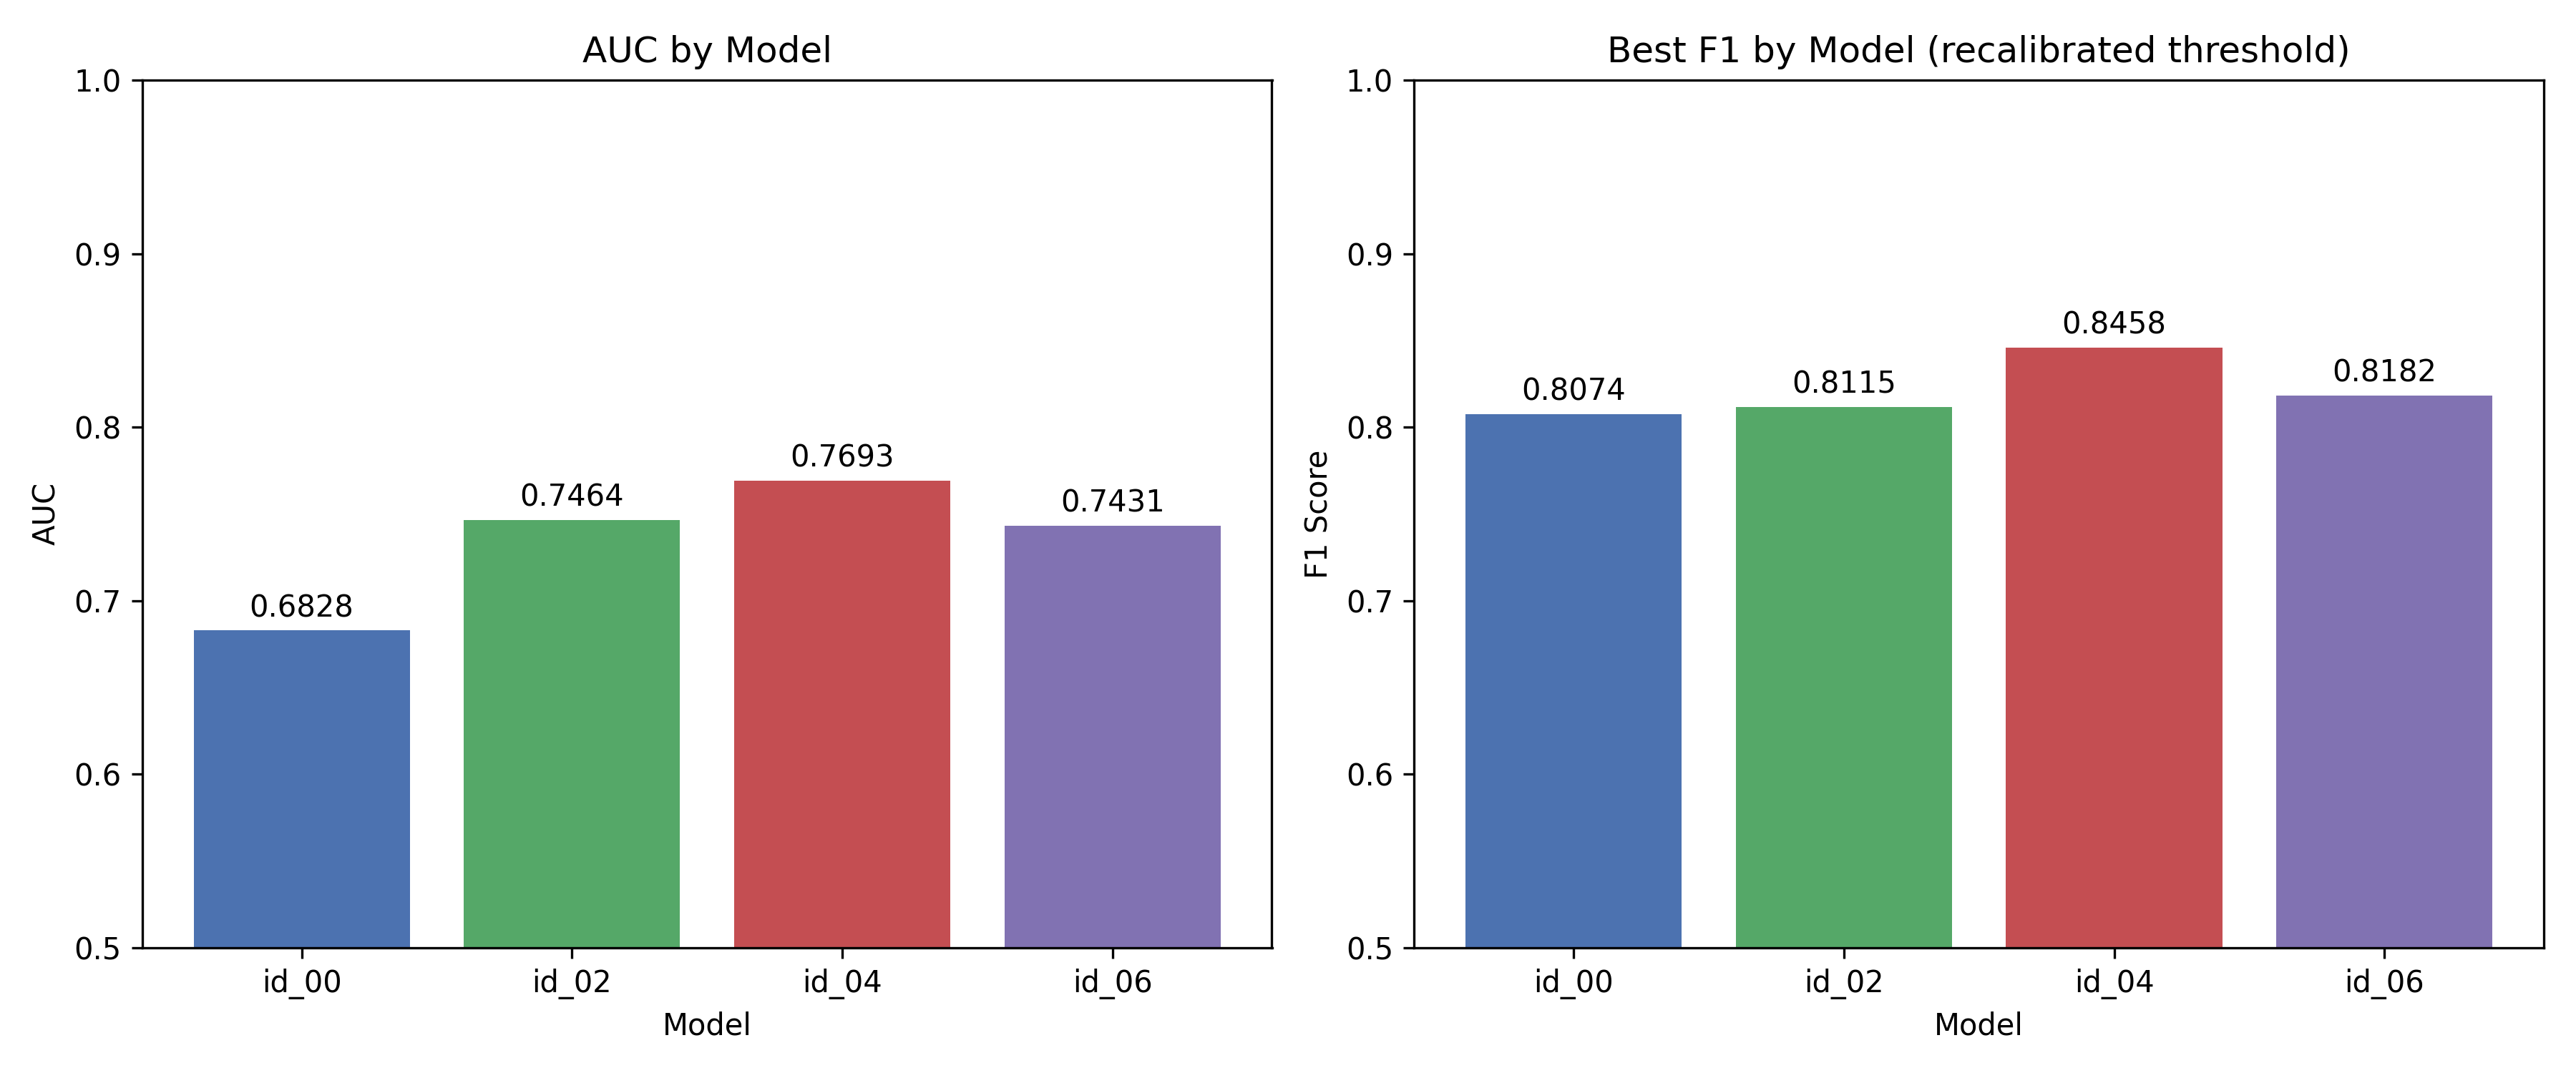
\includegraphics[width=0.95\textwidth]{figures/model_comparison_auc_f1.png}
    \caption{AUC and best-threshold F1 score comparison across four pretrained baseline models.}
    \label{fig:auc-f1-bar}
\end{figure}

\subsubsection{MSE Distribution Analysis}

Fig.~\ref{fig:mse-violin} presents the MSE distributions for normal and abnormal samples under each model. Table~\ref{tab:mse-stats} provides the corresponding statistics.

\begin{table}[htbp]
\centering
\caption{MSE statistics (mean $\pm$ std) for normal and abnormal groups under each model.}
\label{tab:mse-stats}
\begin{tabular}{lcc}
\toprule
Model & Normal (mean $\pm$ std) & Abnormal (mean $\pm$ std) \\
\midrule
id\_00 & $53.20 \pm 25.41$ & $72.74 \pm 30.49$ \\
id\_02 & $44.34 \pm 9.83$  & $56.00 \pm 15.58$ \\
id\_04 & $41.81 \pm 13.91$ & $56.21 \pm 18.51$ \\
id\_06 & $57.56 \pm 12.70$ & $70.86 \pm 15.69$ \\
\bottomrule
\end{tabular}
\end{table}

\begin{figure}[htbp]
    \centering
    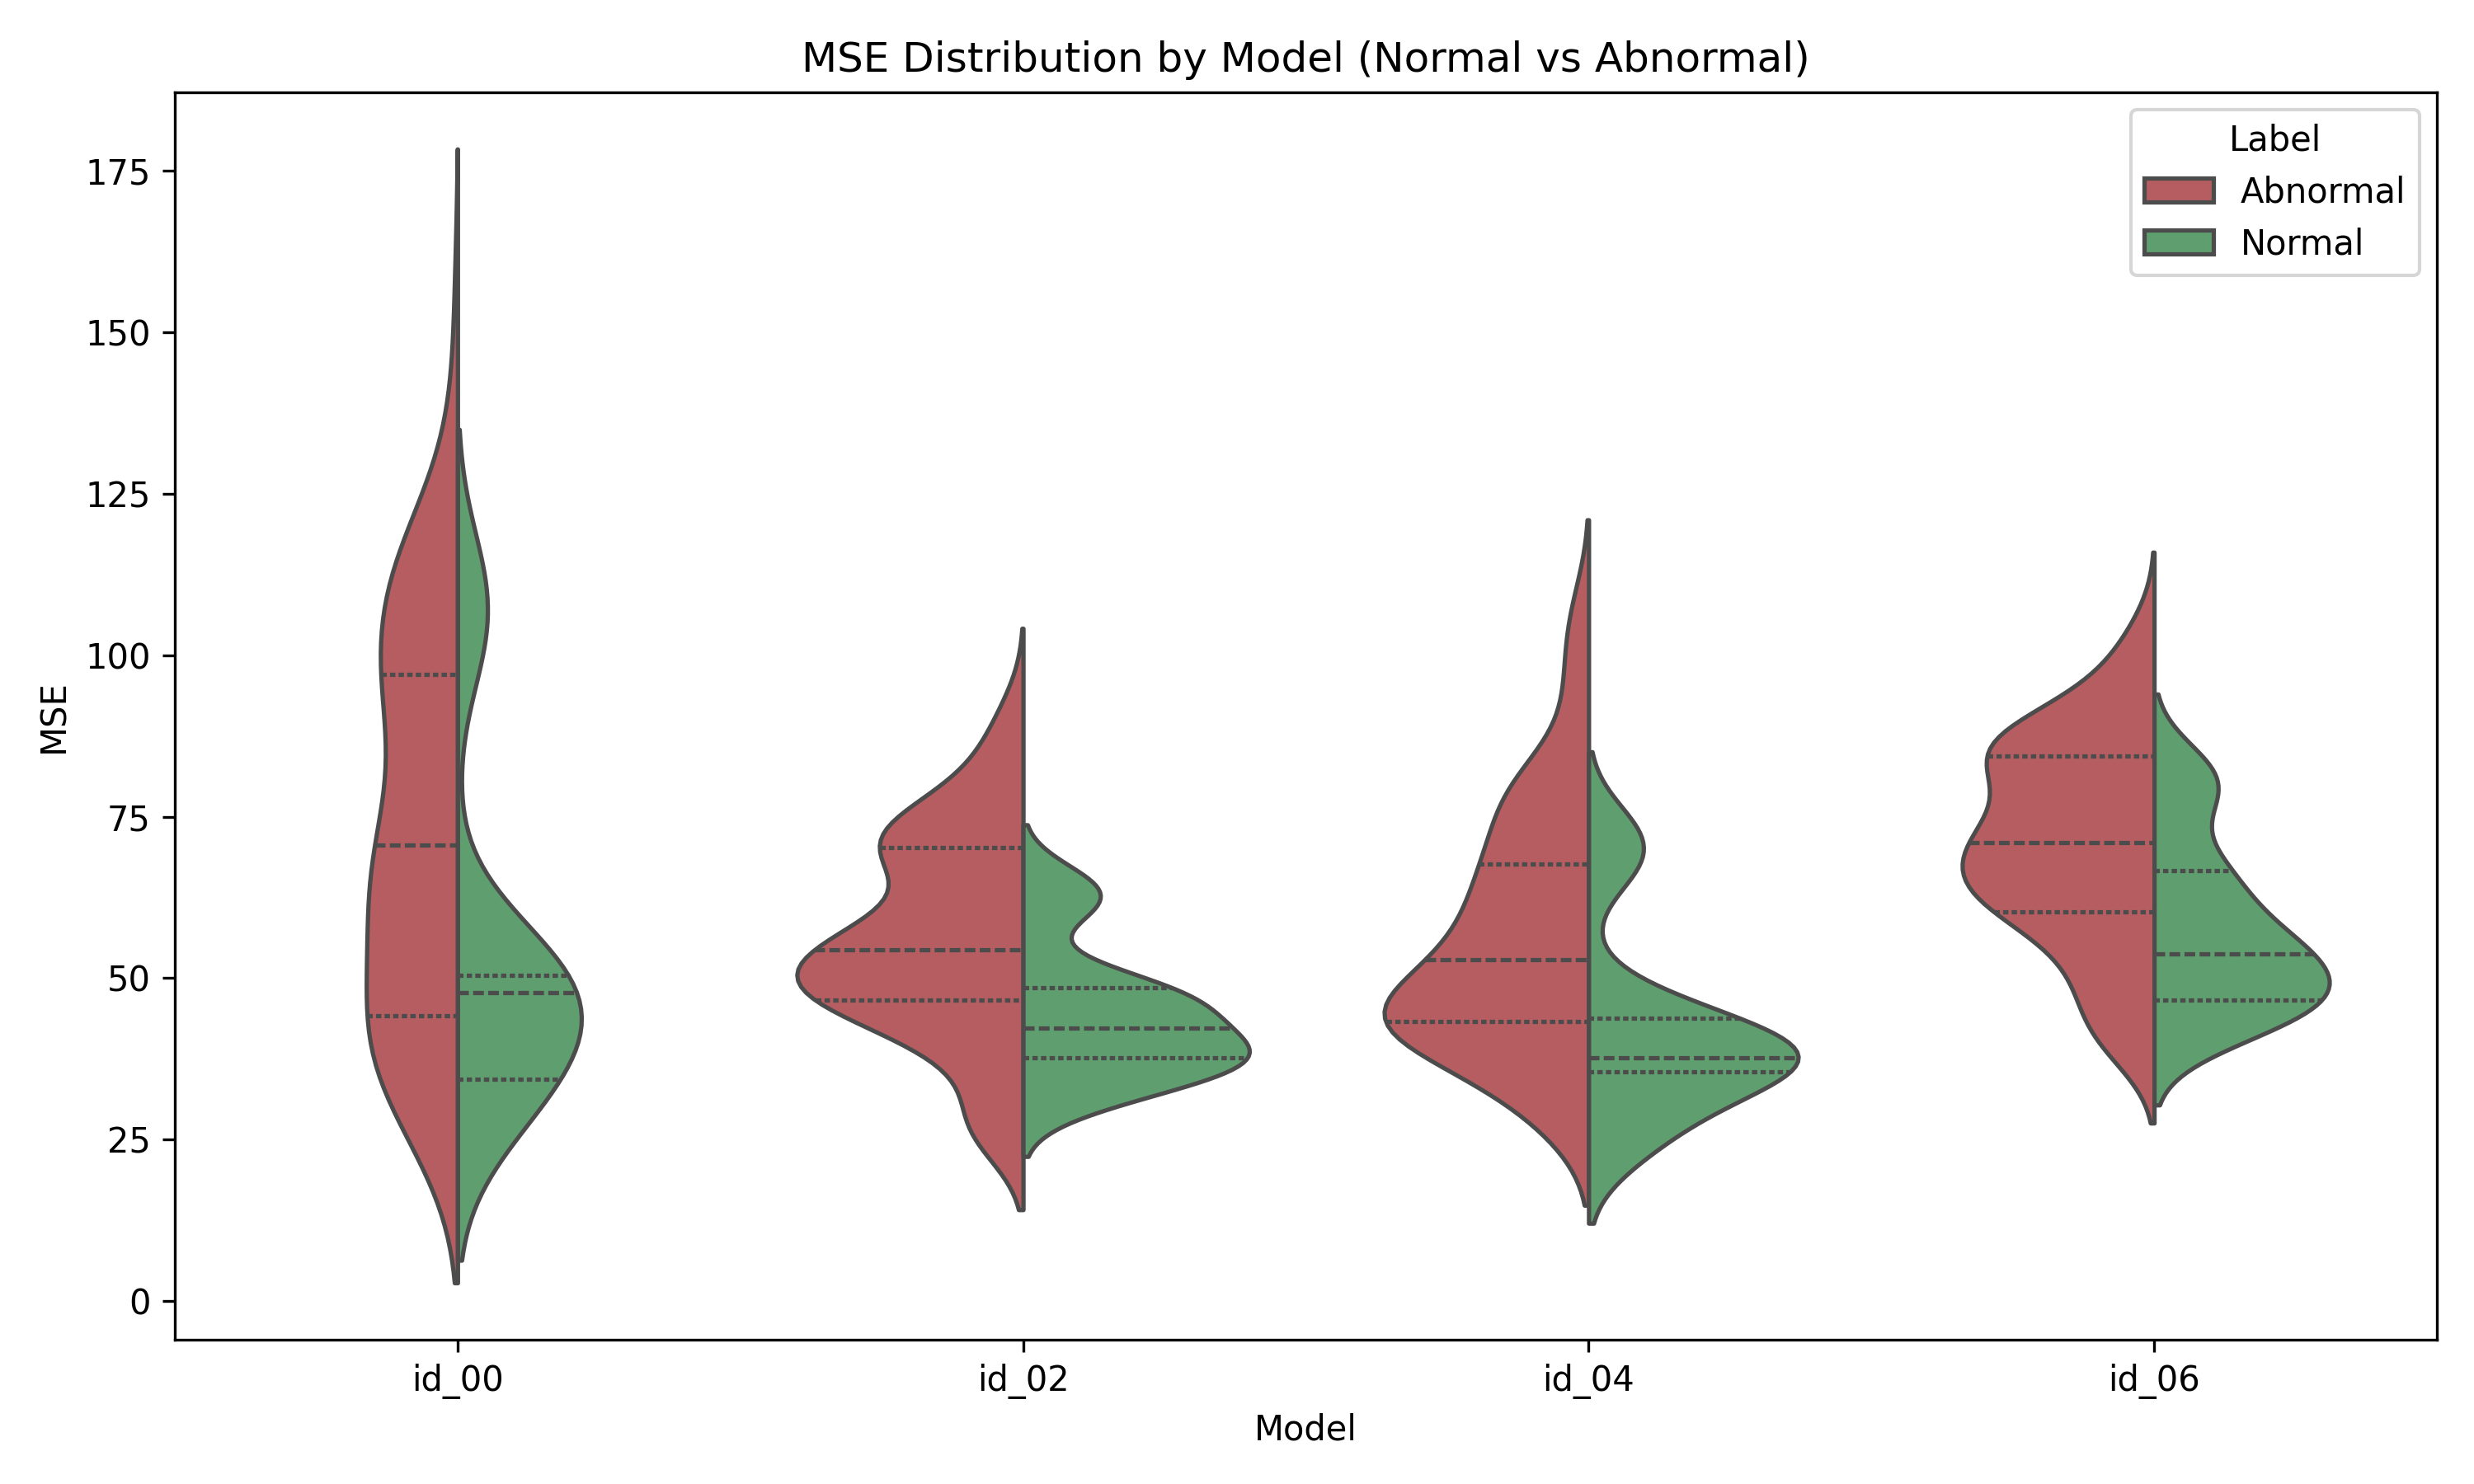
\includegraphics[width=0.85\textwidth]{figures/model_comparison_mse_violin.png}
    \caption{Violin plot of MSE distributions for normal vs.\ abnormal samples across all four models.}
    \label{fig:mse-violin}
\end{figure}

Several observations emerge from the distribution analysis:

\begin{itemize}
    \item All four models produce substantially higher MSE values on our target data than on the original MIMII source domain (e.g., the original threshold for \texttt{id\_06} is 7.01, whereas the mean MSE on our data ranges from 41--73), confirming the presence of significant domain shift.
    \item \texttt{id\_00} exhibits the highest variance in both groups ($\sigma_{\text{normal}} = 25.41$), which explains its lower AUC --- the broad overlap between normal and abnormal distributions impairs separability.
    \item \texttt{id\_02} achieves the tightest normal-class distribution ($\sigma = 9.83$), but its abnormal-class mean is only moderately elevated, resulting in a smaller margin than \texttt{id\_04}.
    \item \texttt{id\_04} offers the best trade-off: a relatively compact normal distribution with a sufficiently large mean gap ($\Delta\mu = 14.40$), leading to the best AUC.
\end{itemize}

\begin{figure}[htbp]
    \centering
    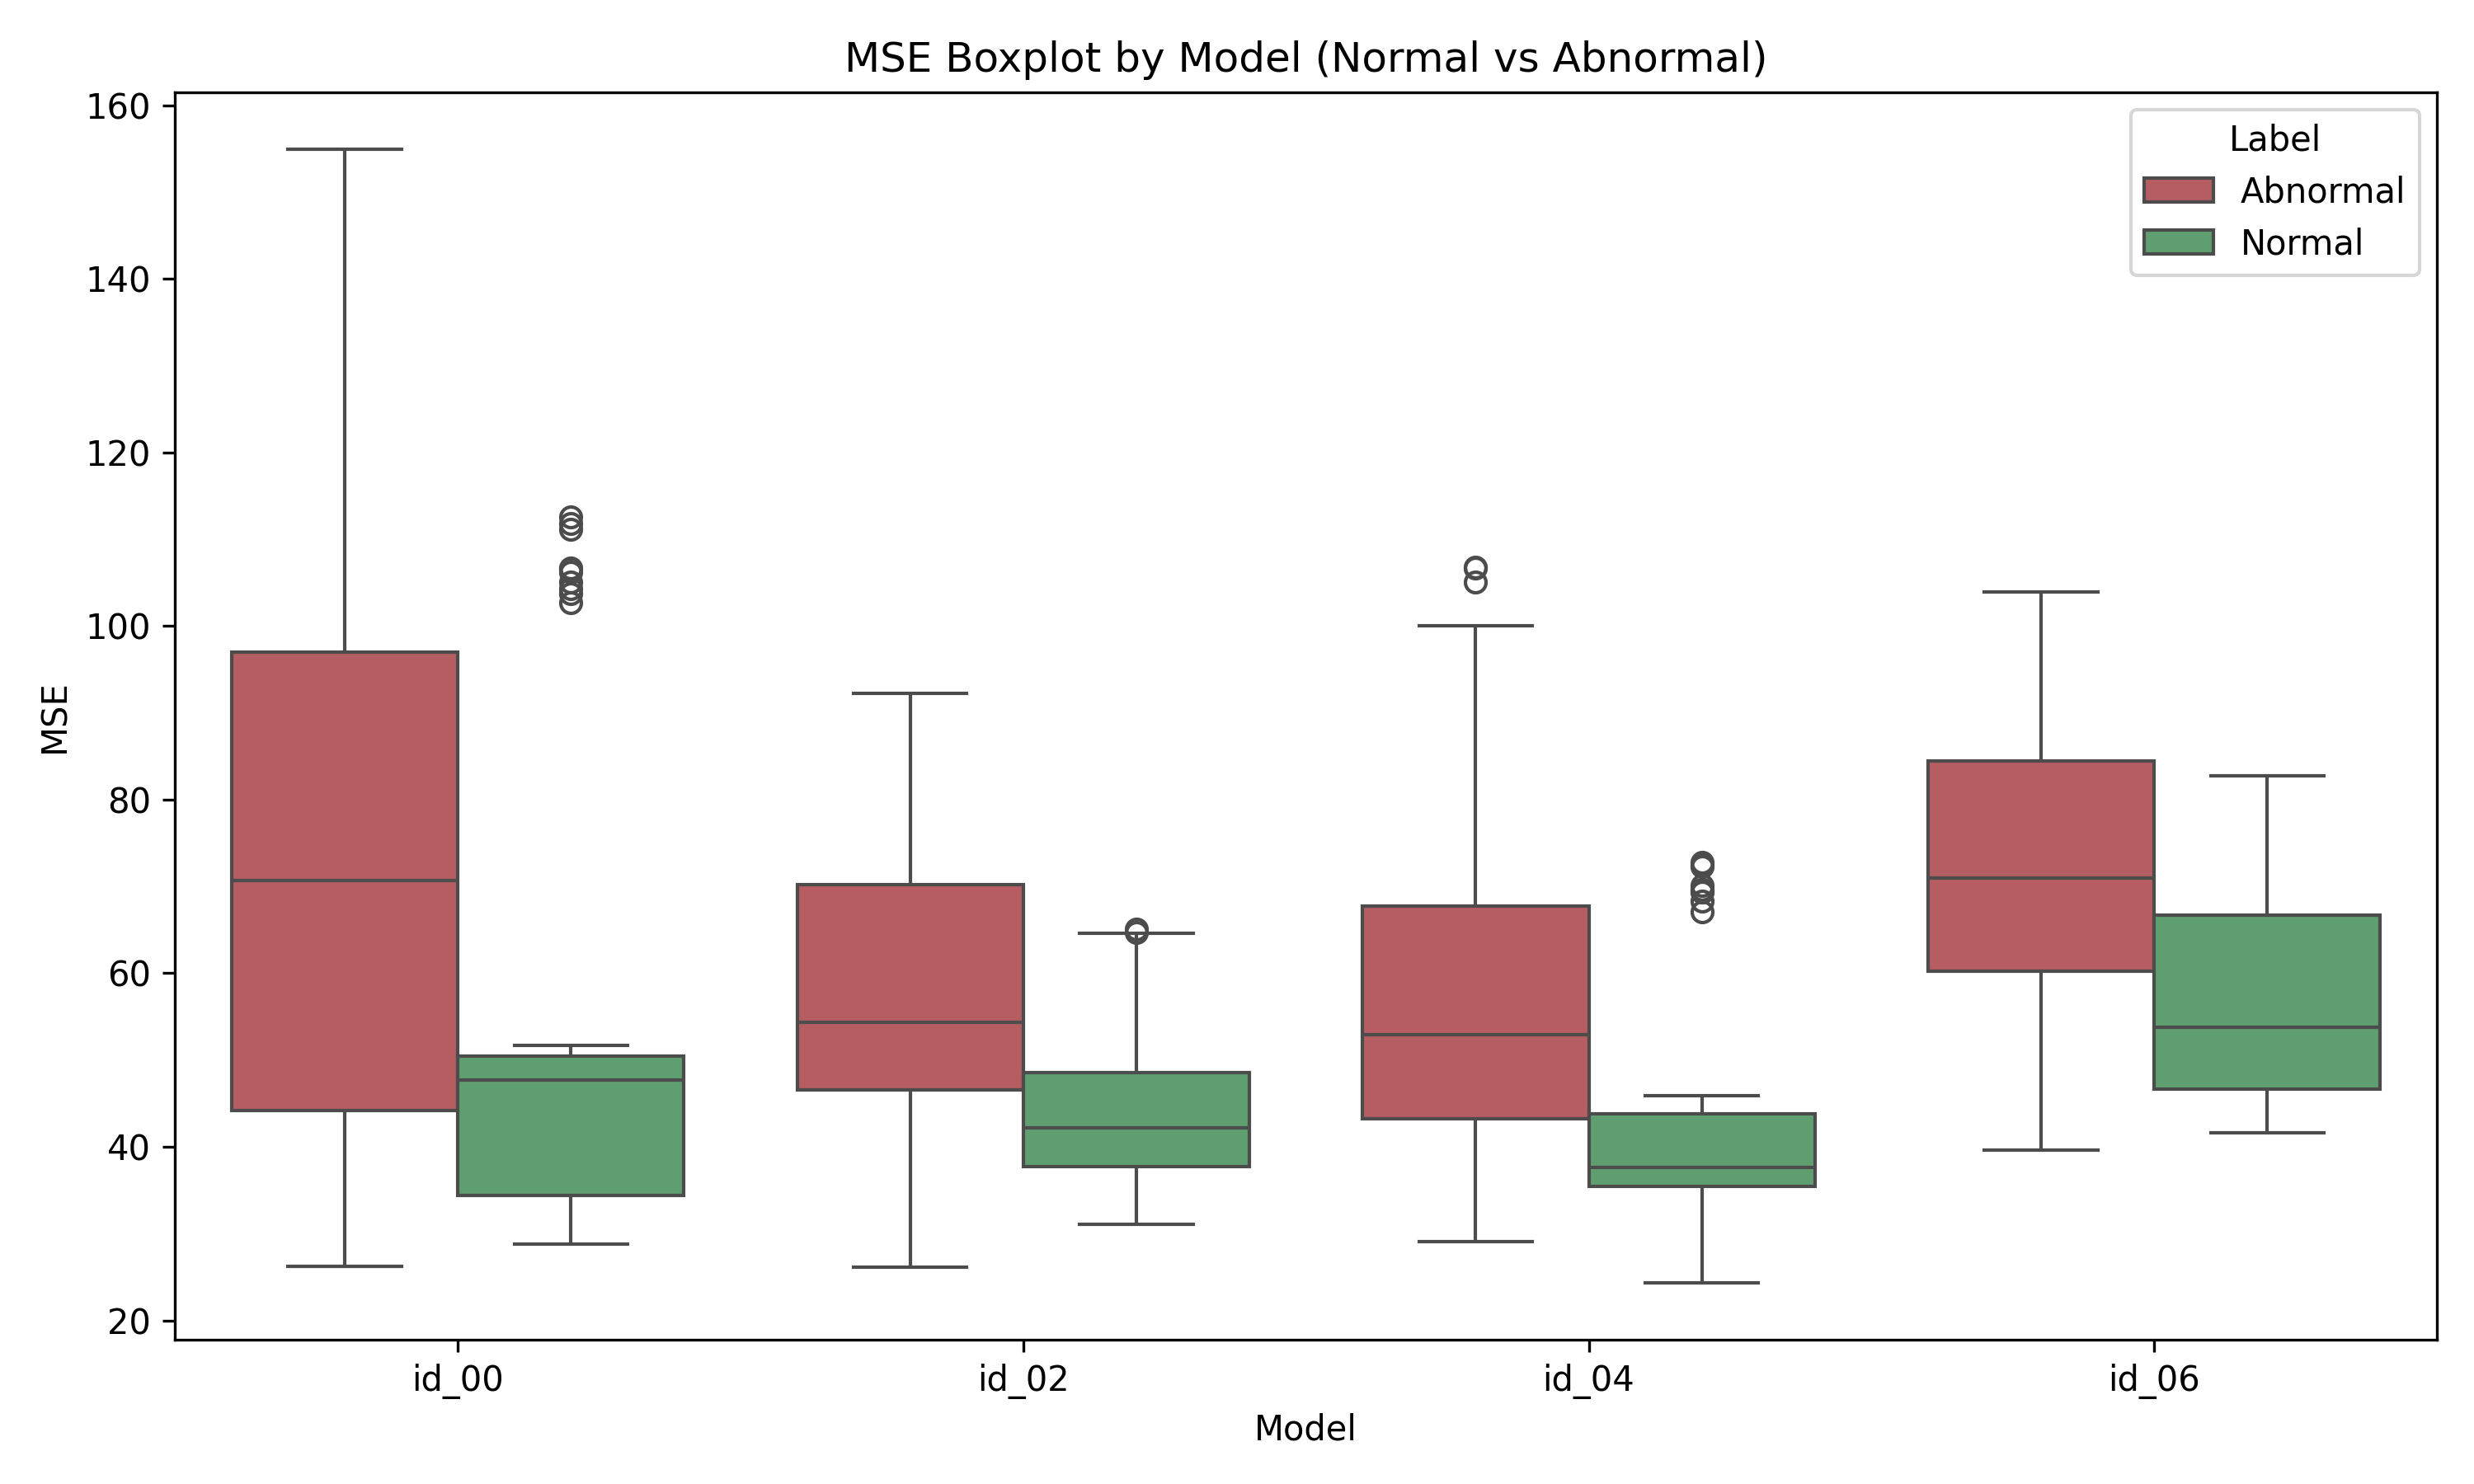
\includegraphics[width=0.85\textwidth]{figures/model_comparison_mse_boxplot.png}
    \caption{Boxplot of MSE grouped by label (Normal vs.\ Abnormal) for each model.}
    \label{fig:mse-boxplot}
\end{figure}

\subsubsection{Breakdown by Operating Condition}

Fig.~\ref{fig:mse-condition} shows the MSE distributions broken down by the three operating conditions for each model. Across all four models, a consistent pattern emerges:

\begin{itemize}
    \item \textbf{Imbalance} consistently produces the highest MSE, suggesting that rotational imbalance introduces the most spectrally distinctive acoustic signatures relative to the source-domain training data.
    \item \textbf{Blocked} shows intermediate MSE values, indicating that airflow obstruction creates detectable but less pronounced spectral deviations.
    \item \textbf{Normal} has the lowest MSE, as expected for a reconstruction-based anomaly detector.
\end{itemize}

This ordering holds across all four models, confirming that the phenomenon is condition-driven rather than model-specific.

\begin{figure}[htbp]
    \centering
    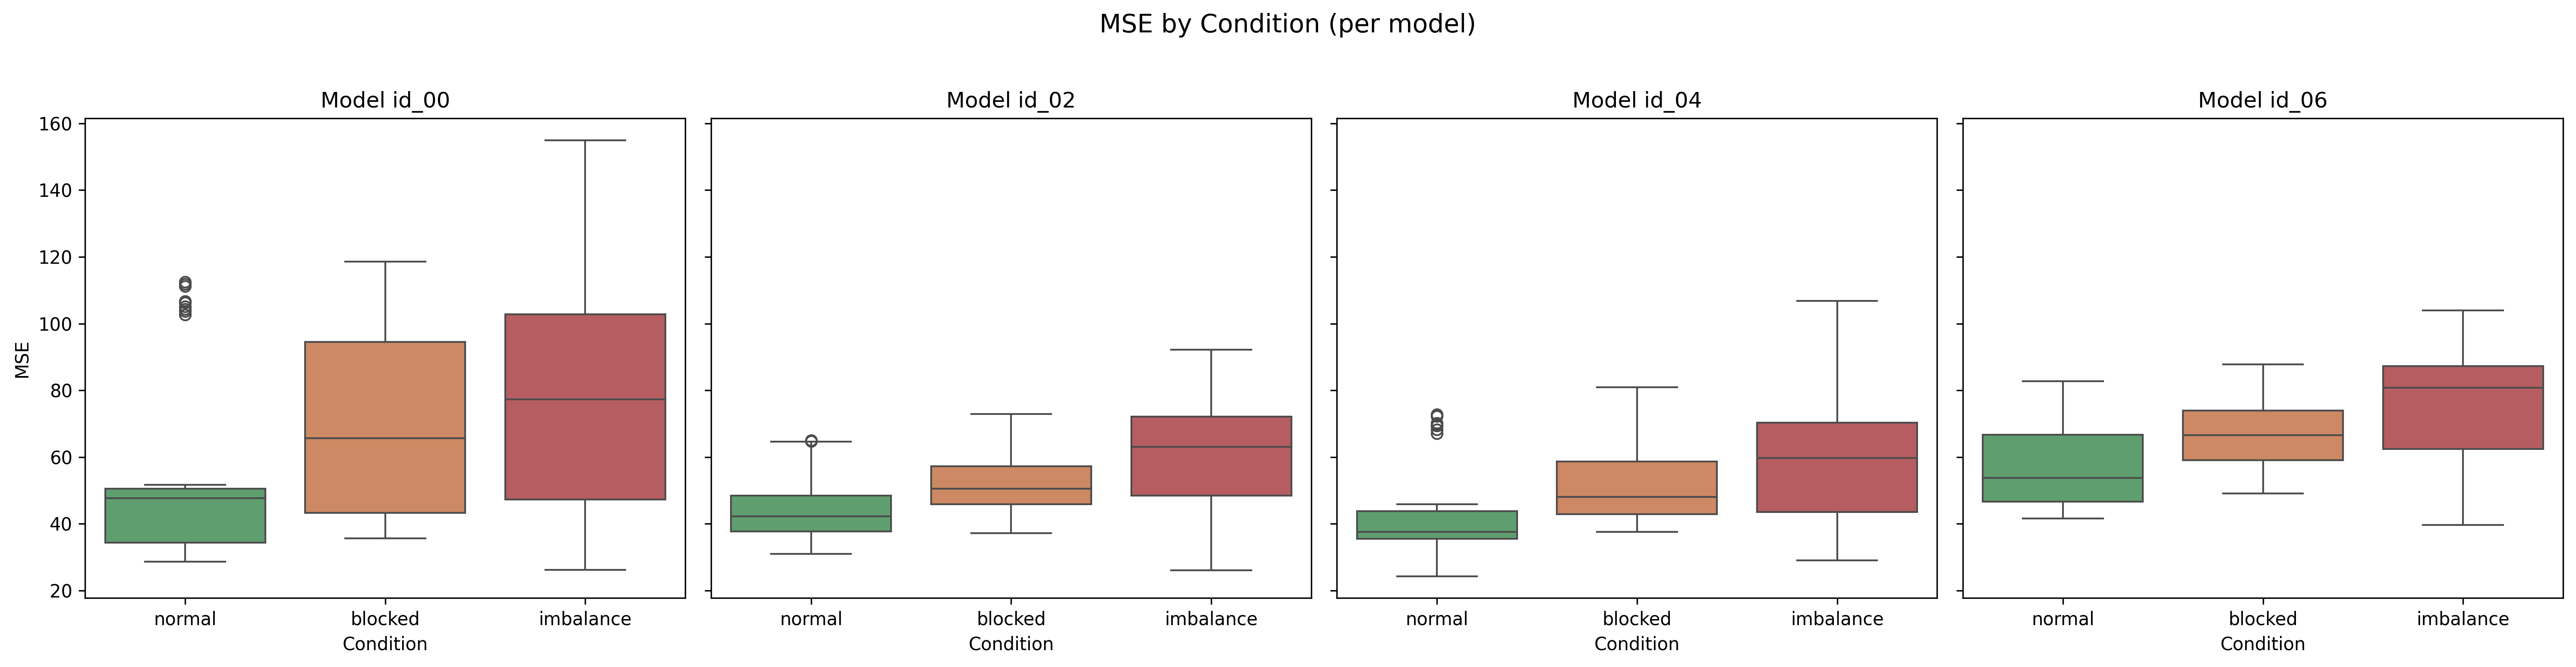
\includegraphics[width=\textwidth]{figures/model_comparison_mse_by_condition.png}
    \caption{MSE distribution by operating condition (normal, blocked, imbalance) for each model.}
    \label{fig:mse-condition}
\end{figure}

\subsubsection{Effect of Voltage Level}

Fig.~\ref{fig:mse-voltage} illustrates the effect of supply voltage (4V, 8V, 12V) on reconstruction error. Higher voltage corresponds to higher fan speed, which in turn affects the acoustic profile. In general, 12V tends to produce elevated MSE across all models, likely because higher rotational speed amplifies both normal operational noise and anomaly-induced spectral differences.

\begin{figure}[htbp]
    \centering
    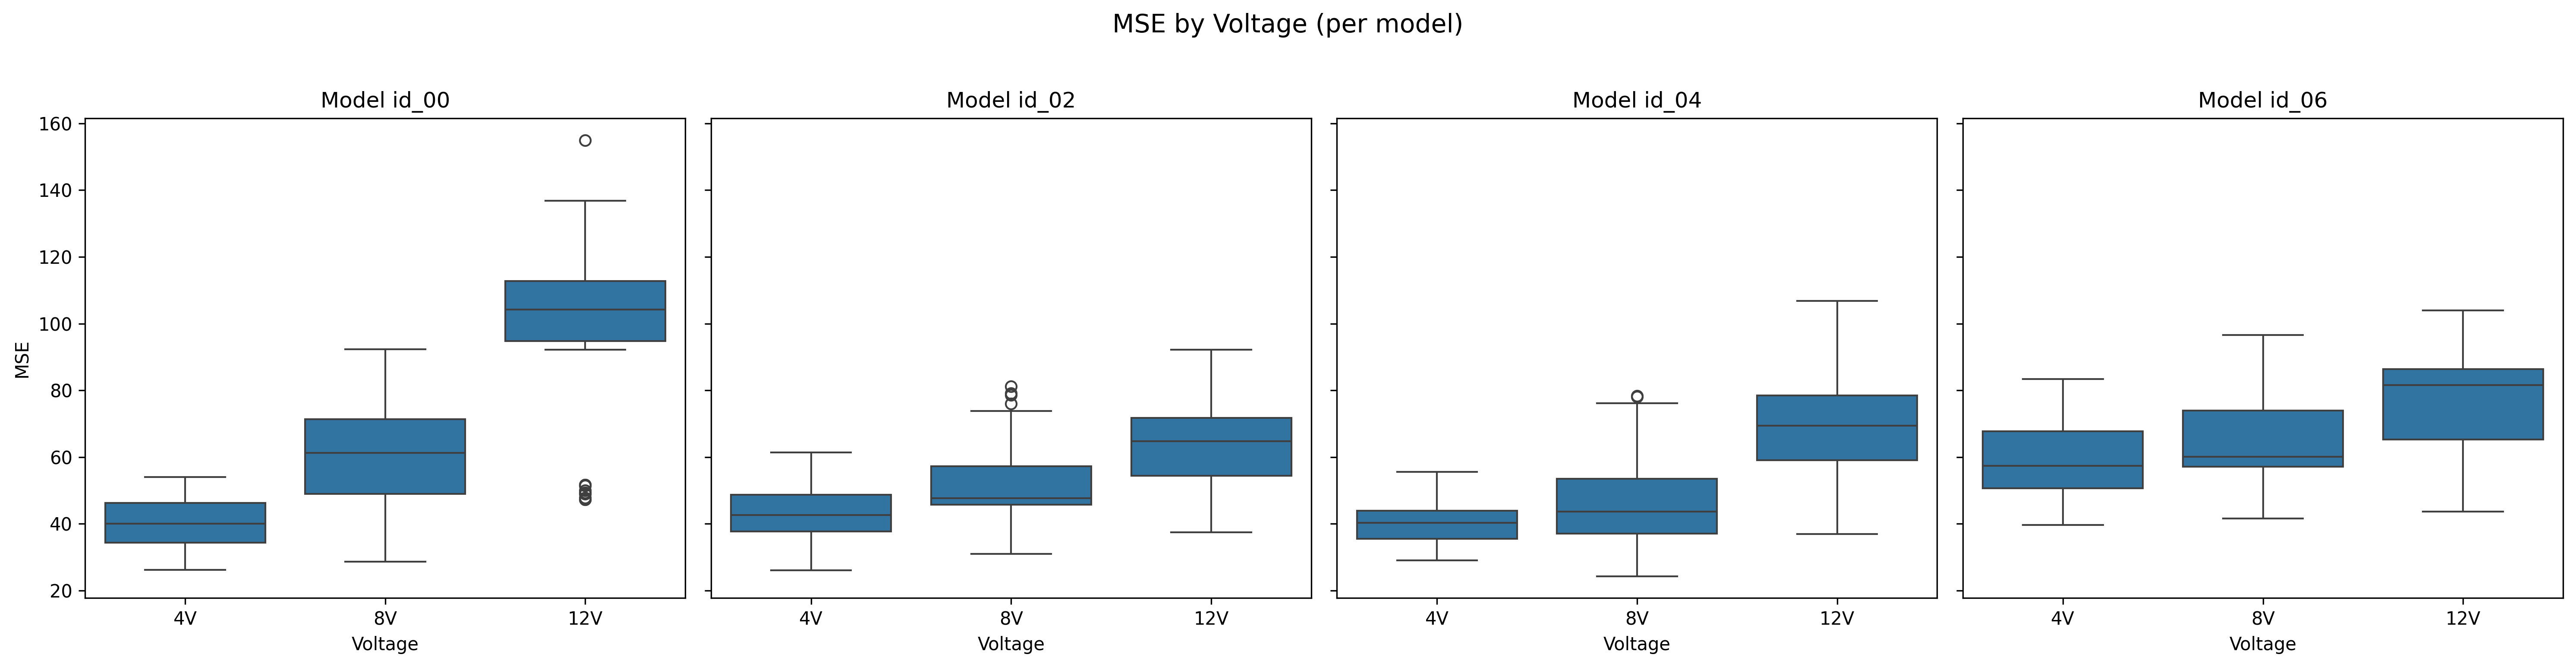
\includegraphics[width=\textwidth]{figures/model_comparison_mse_by_voltage.png}
    \caption{MSE distribution by voltage level (4V, 8V, 12V) for each model.}
    \label{fig:mse-voltage}
\end{figure}

\subsubsection{Effect of Noise Environment}

Fig.~\ref{fig:mse-noise} compares MSE under quiet and noise conditions. A counterintuitive finding persists across all models: the quiet environment produces slightly higher MSE than the noise environment. One plausible explanation is that the MIMII source-domain recordings were collected in a moderately noisy industrial environment; consequently, our noise condition is acoustically closer to the source-domain training distribution, resulting in lower reconstruction error. The quiet condition, being further from the source distribution, incurs a larger domain gap and thus higher MSE.

\begin{figure}[htbp]
    \centering
    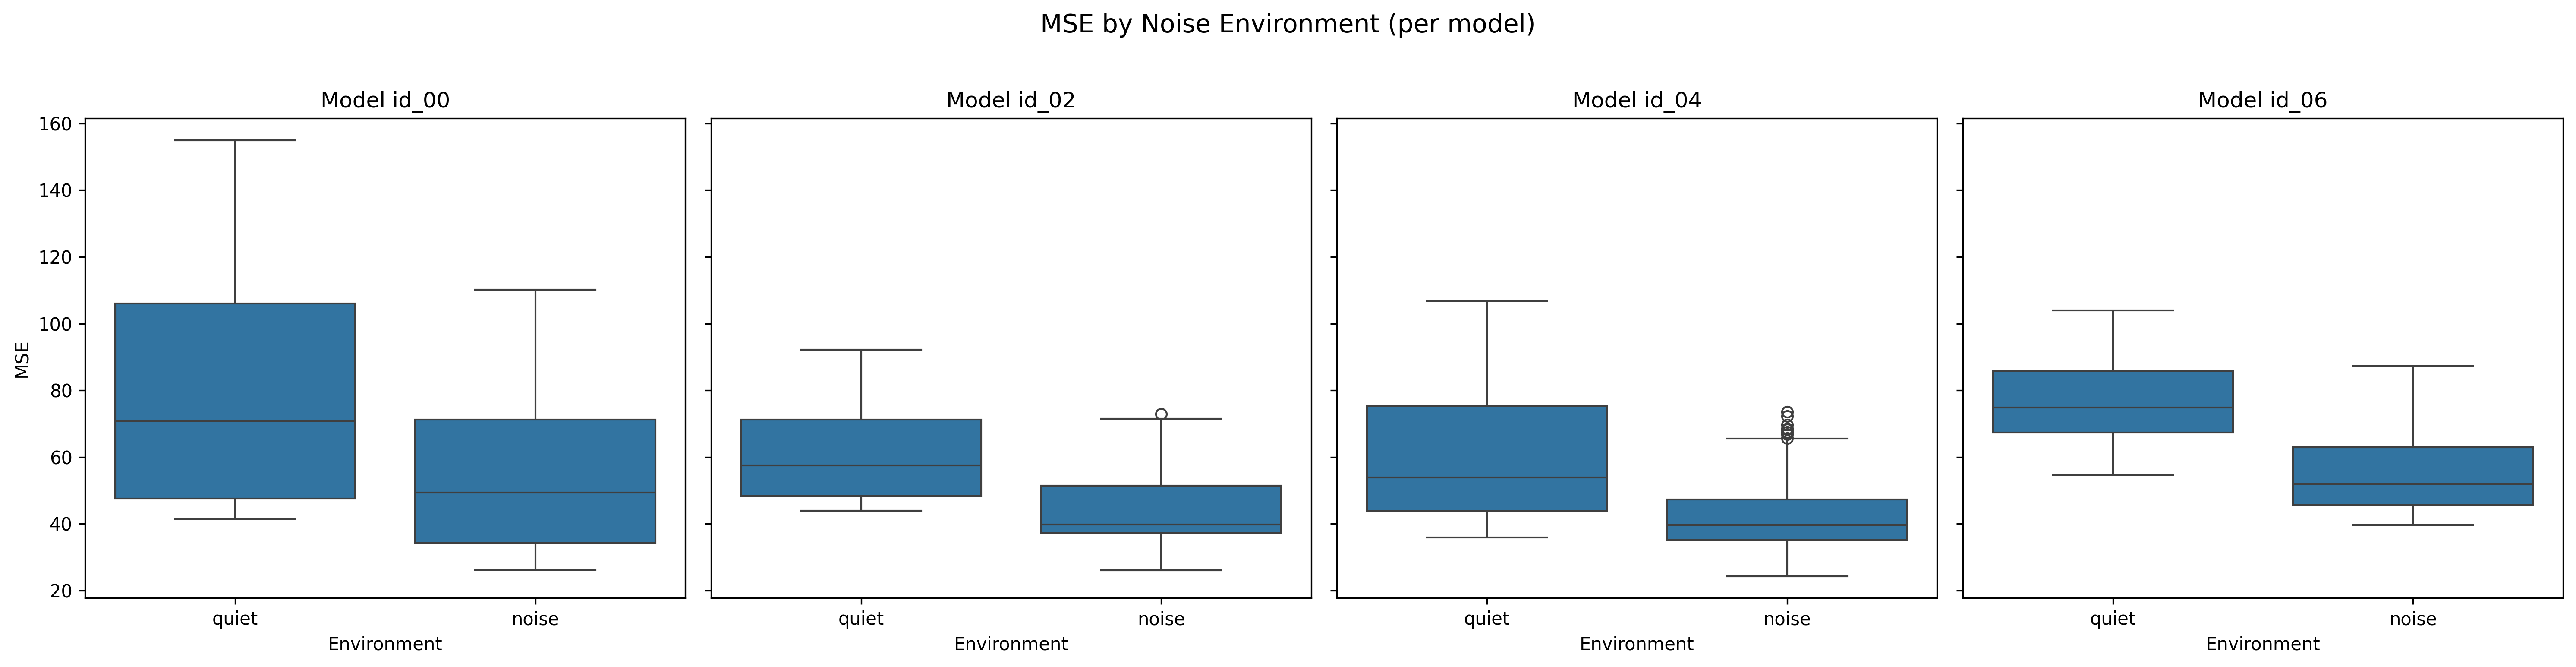
\includegraphics[width=\textwidth]{figures/model_comparison_mse_by_noise.png}
    \caption{MSE distribution by noise environment (quiet vs.\ noise) for each model.}
    \label{fig:mse-noise}
\end{figure}

\subsubsection{Multi-Metric Radar Comparison}

Fig.~\ref{fig:radar} provides a holistic view of all five classification metrics (AUC, F1, Accuracy, Precision, Recall) on a single radar chart. Model \texttt{id\_04} dominates on all axes except precision, where \texttt{id\_06} is marginally higher (0.8115 vs.\ 0.8045). This confirms that \texttt{id\_04} is the most suitable pretrained baseline for subsequent experiments.

\begin{figure}[htbp]
    \centering
    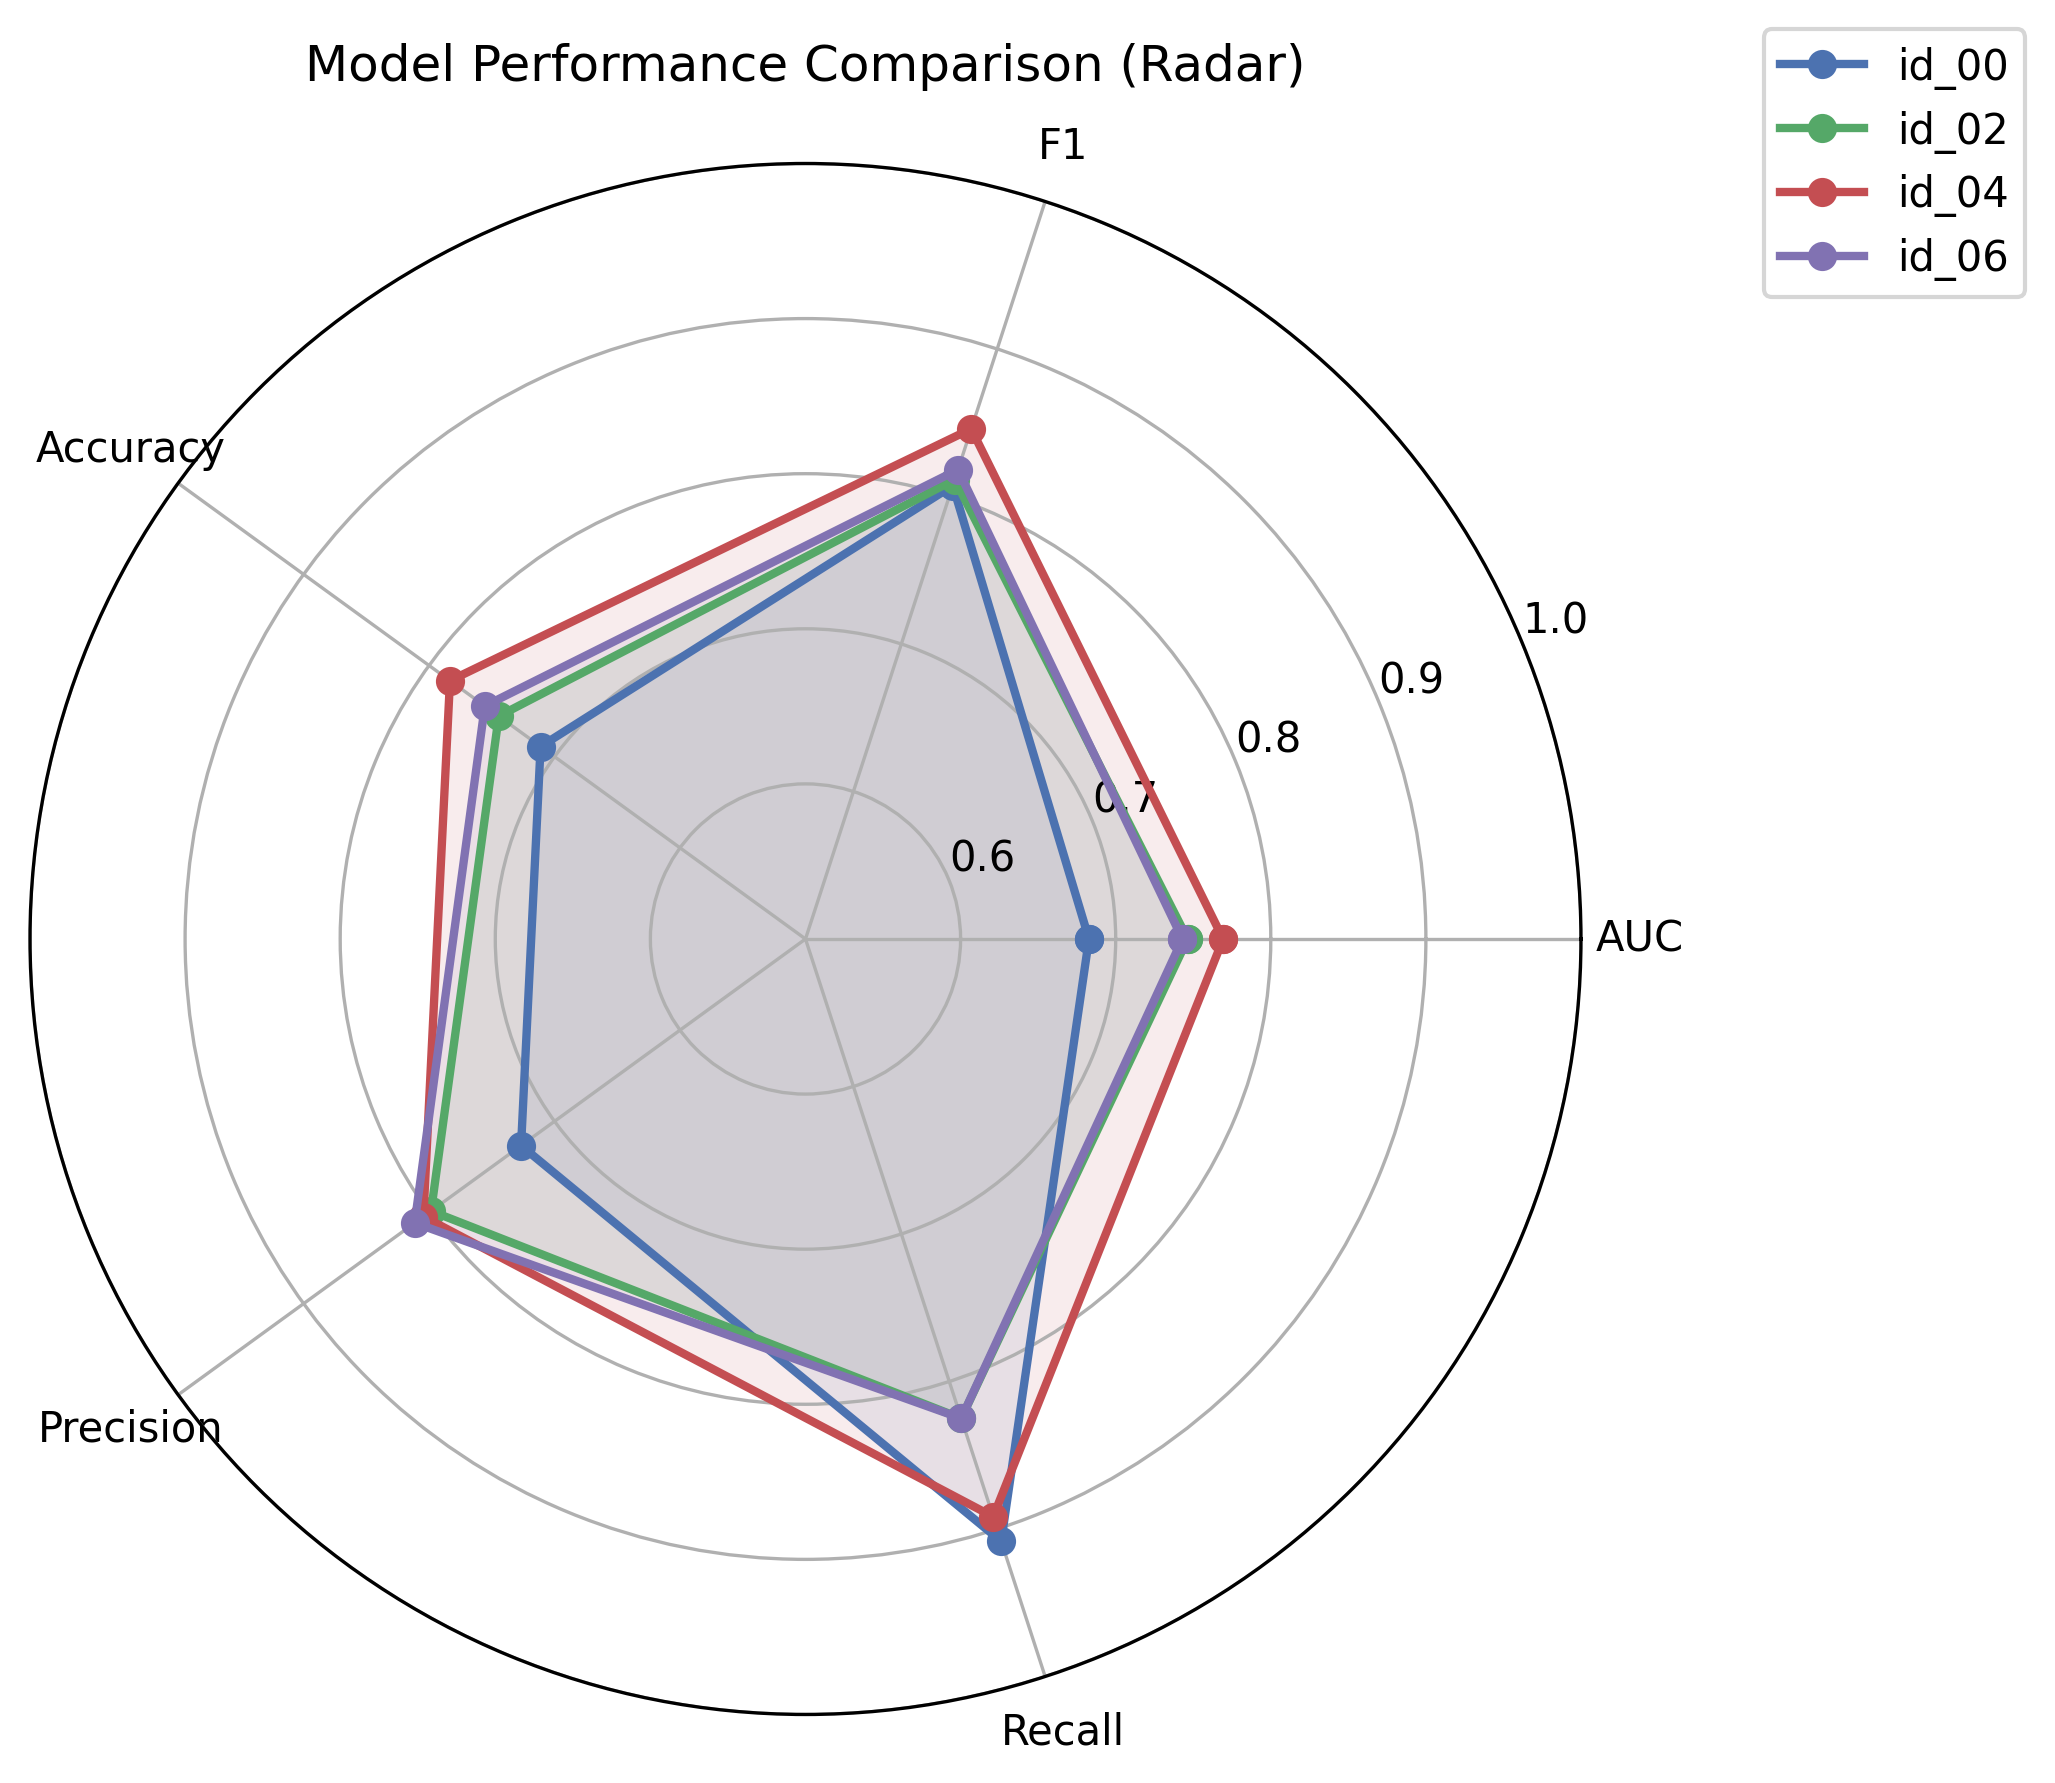
\includegraphics[width=0.6\textwidth]{figures/model_comparison_radar.png}
    \caption{Radar chart comparing five classification metrics across all four models.}
    \label{fig:radar}
\end{figure}

\subsubsection{Cross-Model Summary}

The cross-model evaluation yields three key findings:
\begin{enumerate}
    \item \textbf{Best transferring model}: \texttt{id\_04} achieves the highest AUC (0.7693) and F1 (0.8458) among all four MIMII baseline models, making it the preferred starting point for downstream adaptation.
    \item \textbf{Domain shift is universal}: All models exhibit MSE scales far above their source-domain thresholds (e.g., original threshold 7.01 vs.\ observed MSE range 35--73), confirming that direct threshold transfer is infeasible.
    \item \textbf{Consistent condition ranking}: The ordering imbalance $>$ blocked $>$ normal in MSE is stable across all models, indicating that the anomaly signal is robust and model-independent.
\end{enumerate}

Based on these results, we select \texttt{id\_04} as the base model for subsequent experiments.


% --------------------------------------------------------
% 4.2 Latent Feature Analysis (from latent_analysis.tex)
% --------------------------------------------------------
\subsection{Latent Feature Analysis and Multi-Class Classification}
\label{sec:latent-analysis}

The baseline autoencoder uses reconstruction error (MSE) as a scalar anomaly score, treating the task as binary detection (normal vs.\ abnormal). However, the 8-dimensional bottleneck layer may encode richer structural information about different operating conditions. In this section, we investigate whether the pretrained latent representations are sufficient to distinguish among \emph{three} operating conditions --- normal, blocked, and imbalance --- without any retraining or fine-tuning.

All experiments in this section use model \texttt{id\_04}, which achieved the highest AUC (0.7693) and F1 (0.8458) in the cross-model evaluation (Section~\ref{sec:cross-model-eval}).

\subsubsection{Latent Feature Extraction}

For each of the 180 audio files, we extract frame-level latent representations by passing the 320-dimensional input vectors through the encoder only:
\begin{equation}
    \mathbf{z}_t = f_{\text{enc}}(\mathbf{x}_t) \in \mathbb{R}^{8}, \quad t = 1, \ldots, T
\end{equation}
where $T \approx 300$ is the number of frames per 10-second recording. We then compute the file-level latent representation as the temporal mean:
\begin{equation}
    \bar{\mathbf{z}} = \frac{1}{T} \sum_{t=1}^{T} \mathbf{z}_t \in \mathbb{R}^{8}
\end{equation}
This yields a single 8-dimensional feature vector per audio file, which serves as input to both visualization and classification.

\subsubsection{Per-Dimension Analysis}

Before examining the latent space globally, we inspect the activation patterns of each dimension individually. Fig.~\ref{fig:latent-dims} shows box plots of the 8 latent dimensions grouped by operating condition.

\begin{figure}[htbp]
    \centering
    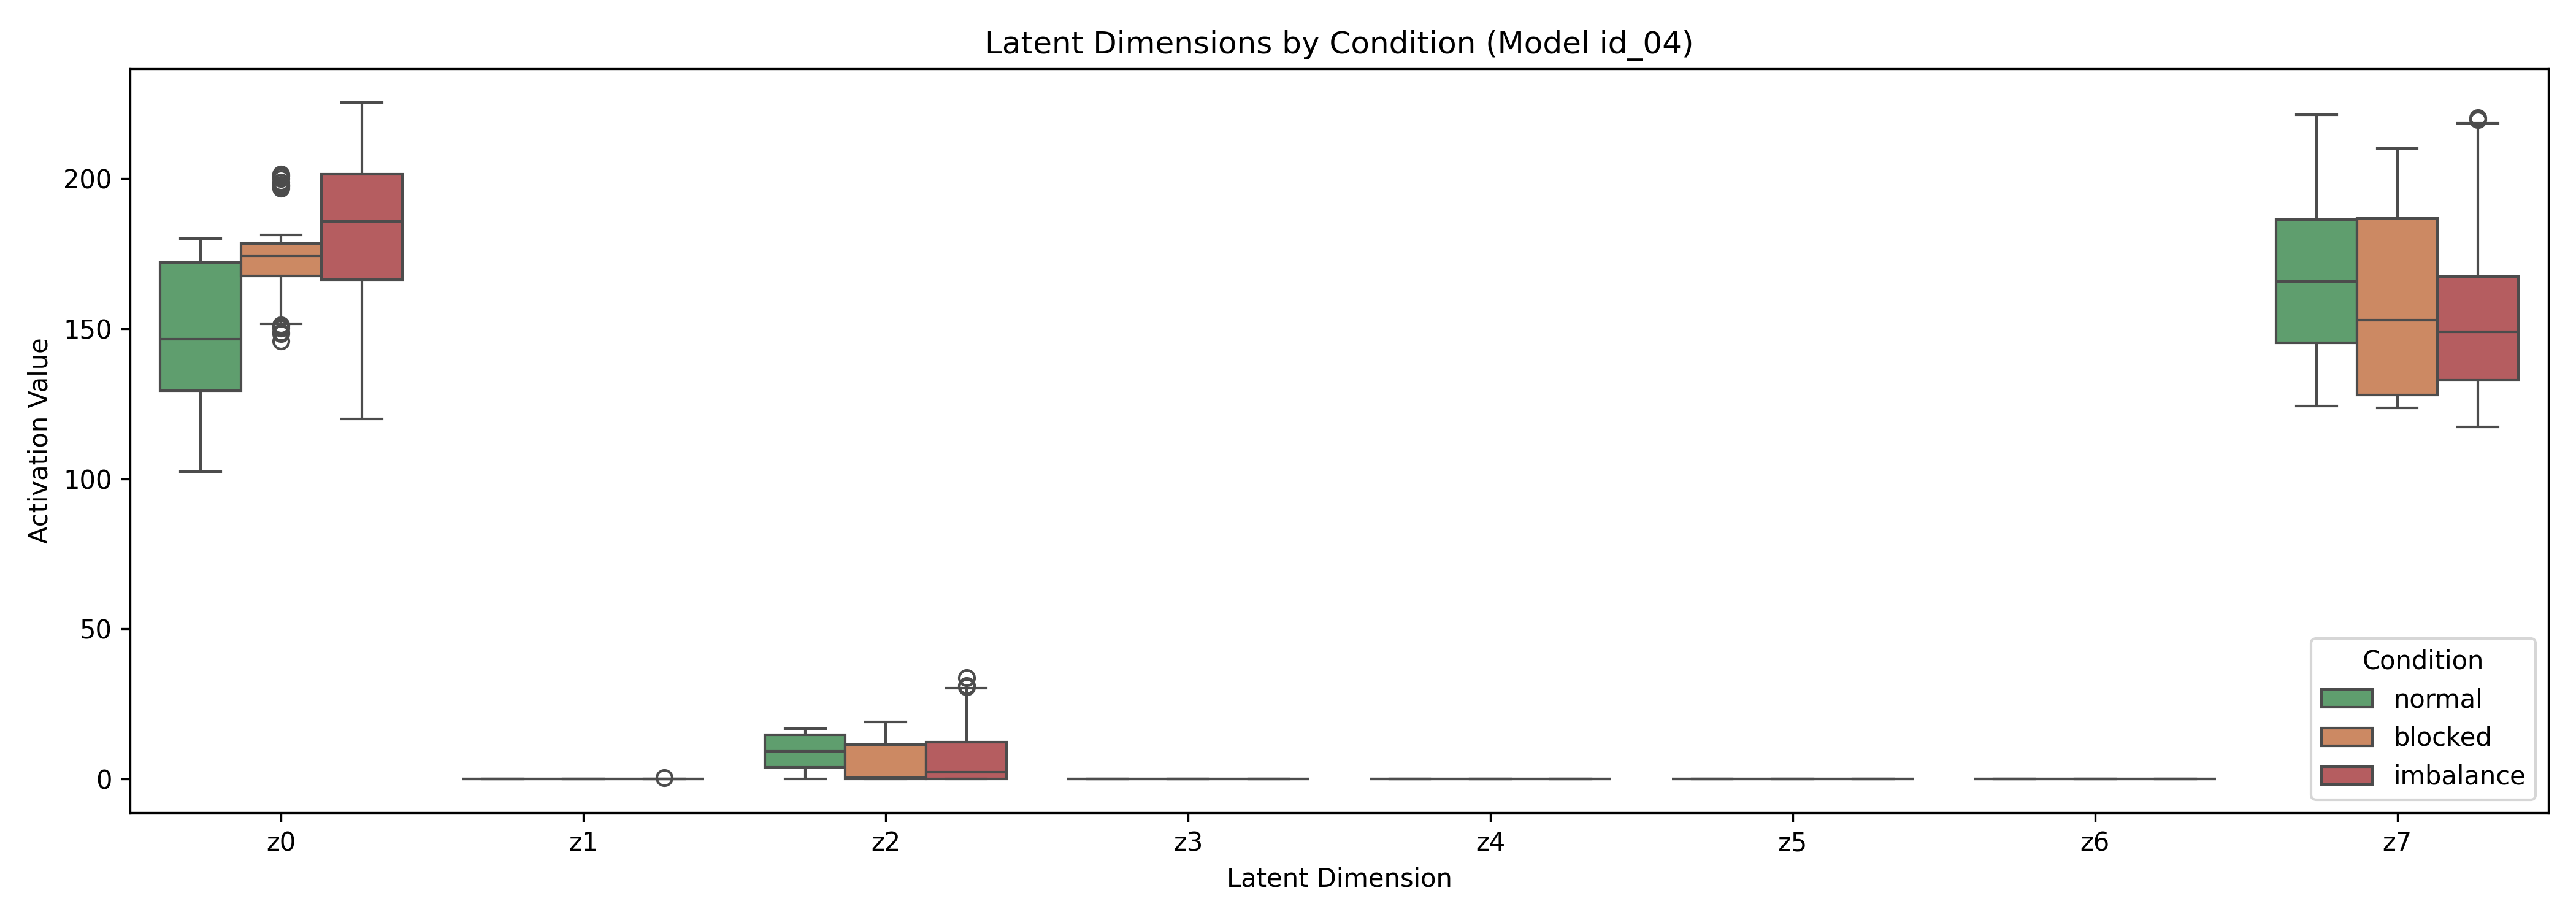
\includegraphics[width=\textwidth]{figures/latent_dimensions_by_condition_id_04.png}
    \caption{Activation values of each latent dimension, grouped by condition. Only dimensions $z_0$ and $z_7$ exhibit non-zero activations; dimensions $z_1$ through $z_6$ are effectively dead.}
    \label{fig:latent-dims}
\end{figure}

A striking observation is that \textbf{six out of eight latent dimensions ($z_1$--$z_6$) are effectively dead}, producing zero or near-zero activations across all 180 files. Only two dimensions carry meaningful information:

\begin{itemize}
    \item \textbf{$z_0$}: ranges from approximately 100 to 200, with normal samples clustering lower ($\sim$140) and imbalance samples higher ($\sim$185). Blocked samples fall in between ($\sim$170).
    \item \textbf{$z_7$}: ranges from approximately 120 to 210, showing partial separation between conditions, though with more overlap than $z_0$.
\end{itemize}

This means the pretrained model's 8-dimensional bottleneck is effectively operating as a \textbf{2-dimensional representation}. Despite this extreme compression, the two active dimensions still encode condition-discriminative information, as confirmed by the subsequent t-SNE and classification analyses.

This finding has direct implications for model architecture exploration: the current bottleneck size of 8 contains substantial redundancy, and the dead-neuron pattern (likely caused by the ReLU activation at the bottleneck output) suggests that alternative activations (e.g., LeakyReLU) or different bottleneck sizes may yield more expressive latent representations after fine-tuning.

\subsubsection{t-SNE Visualization}

To visualize the global structure of the 8-dimensional latent space, we apply t-SNE (perplexity = 30, PCA initialization) to project all 180 file-level latent vectors onto a 2D plane.

\paragraph{By operating condition.}
Fig.~\ref{fig:tsne-condition} shows the t-SNE embedding colored by condition. The three classes form clearly separable clusters, with normal (green), blocked (orange), and imbalance (red) occupying distinct regions. Notably, the clusters are not monolithic --- each condition splits into 2--3 sub-clusters, which correspond to different voltage levels. Despite this sub-structure, the inter-class boundaries remain well-defined, with minimal overlap between conditions.

\begin{figure}[htbp]
    \centering
    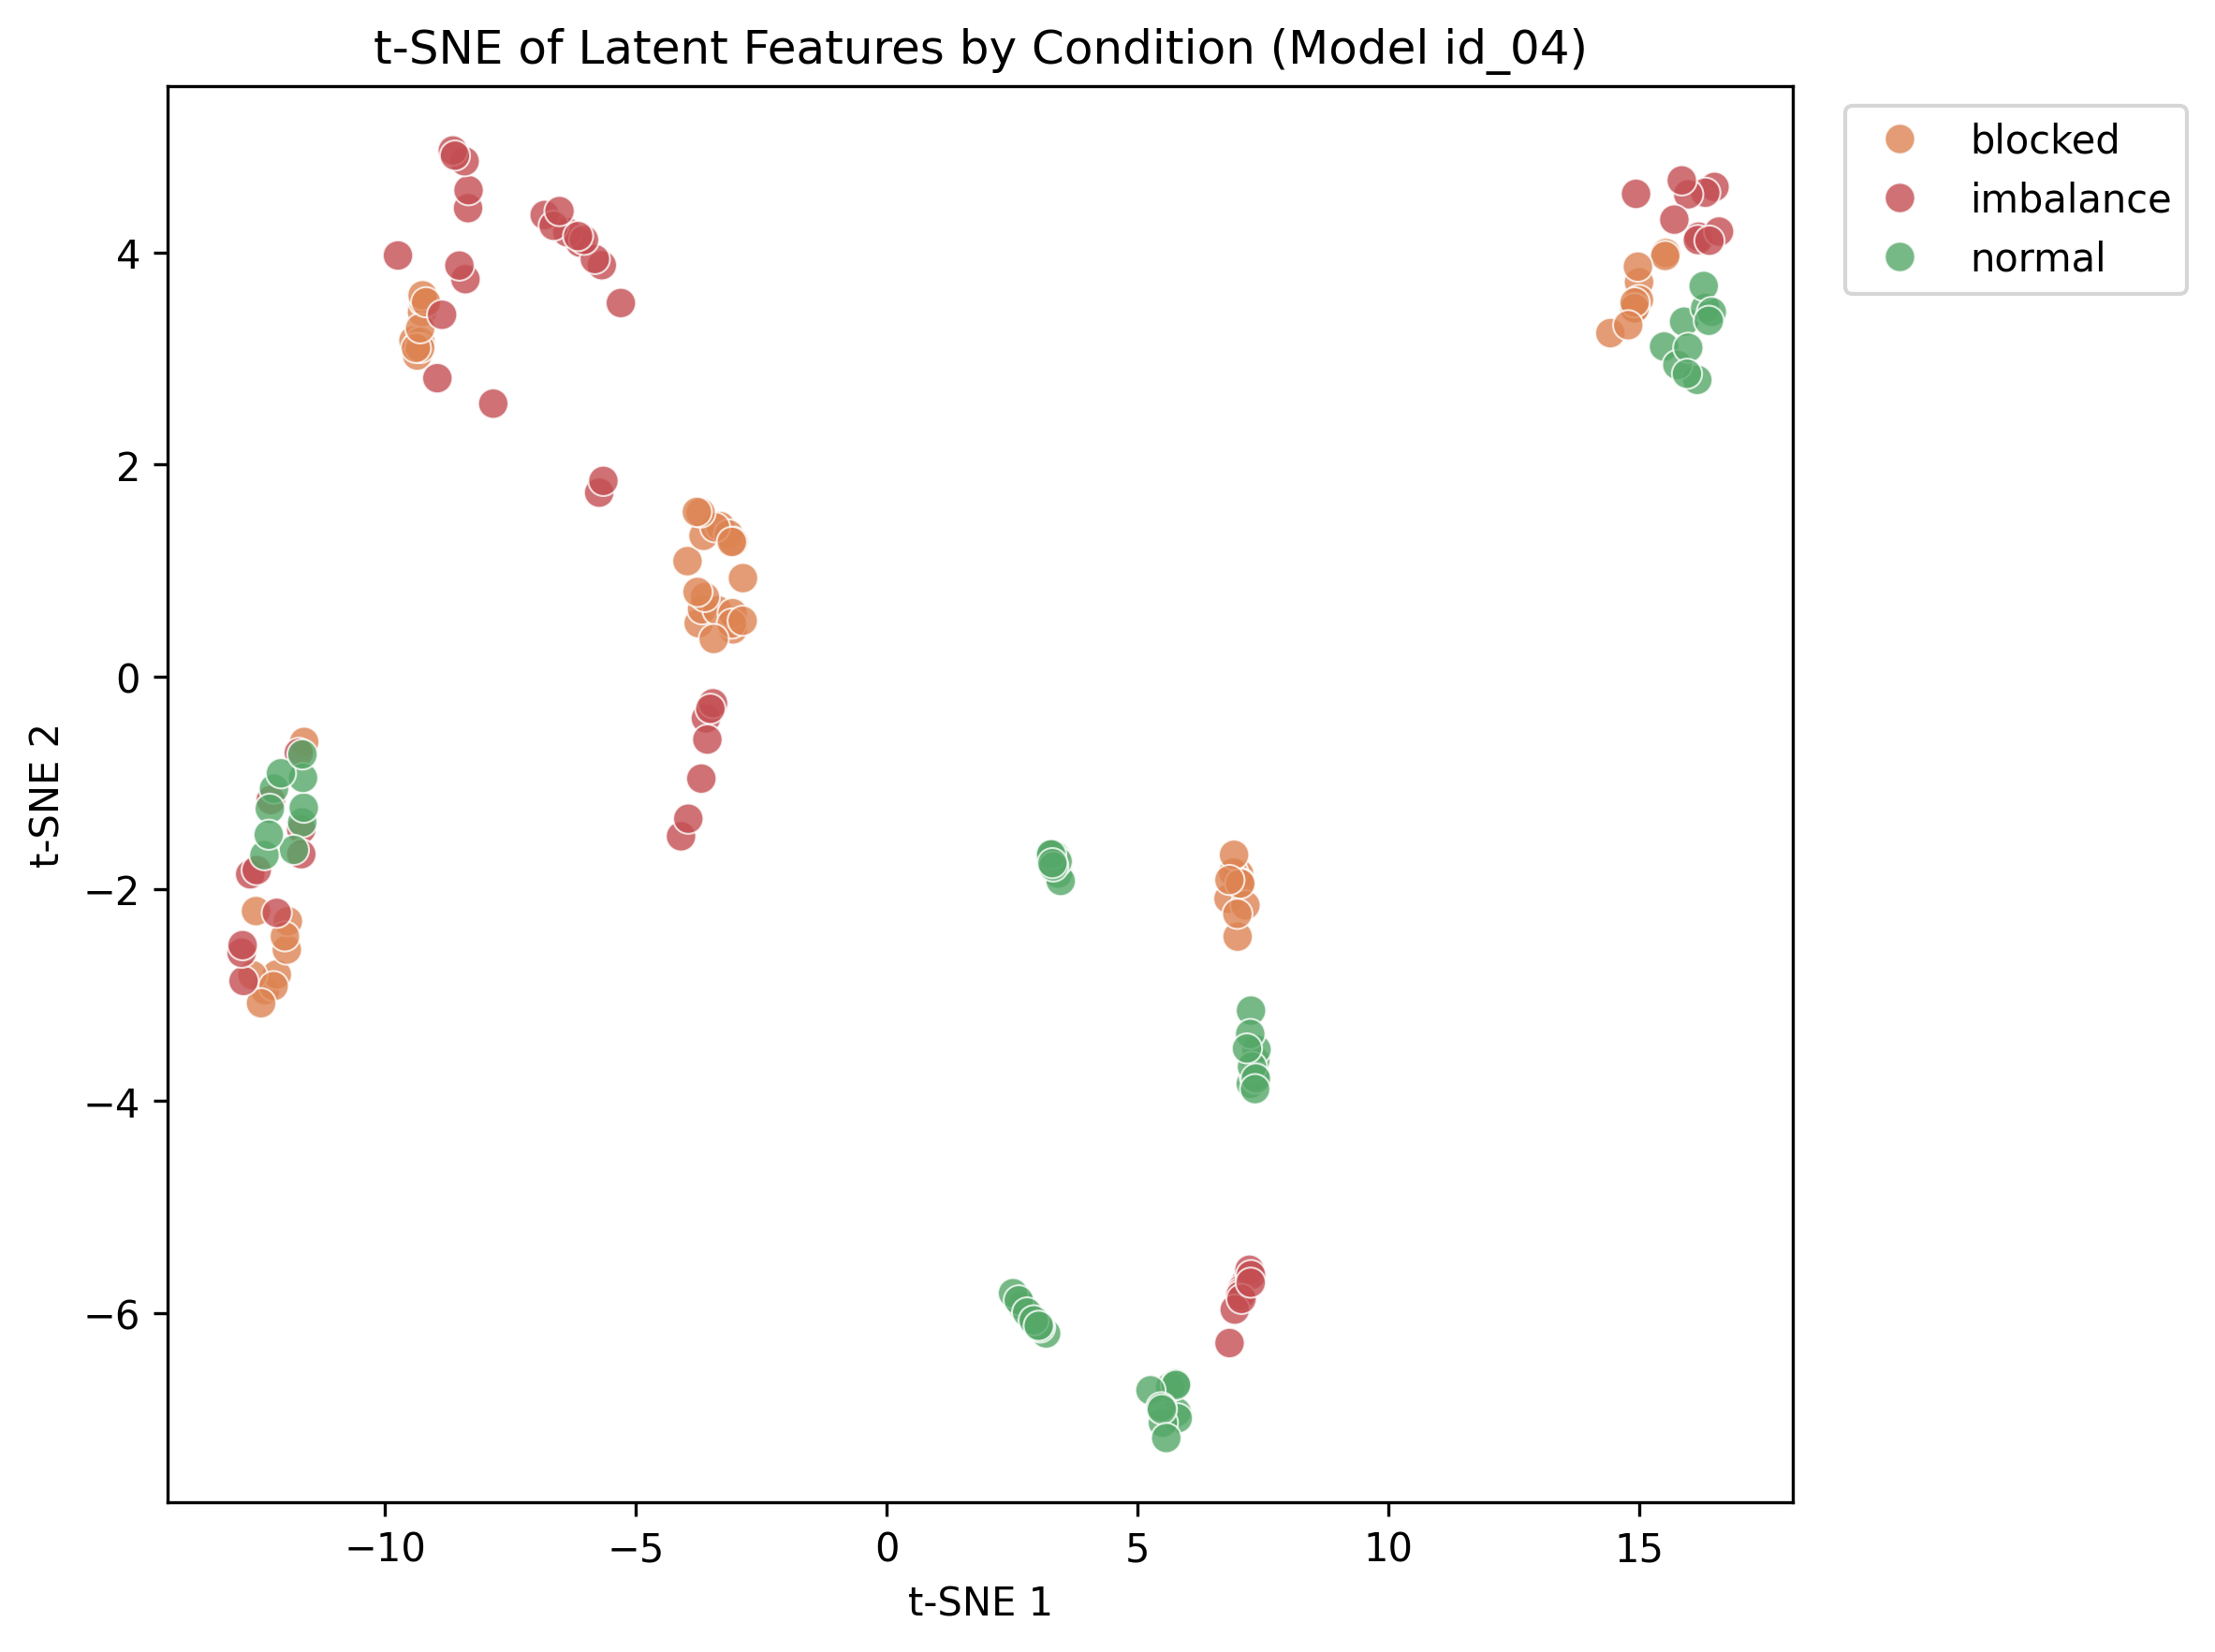
\includegraphics[width=0.75\textwidth]{figures/tsne_by_condition_id_04.png}
    \caption{t-SNE visualization of 8-dim latent features, colored by operating condition. The three classes form clearly separable clusters with distinct sub-structure.}
    \label{fig:tsne-condition}
\end{figure}

\paragraph{By voltage level.}
Fig.~\ref{fig:tsne-voltage} reveals that the sub-cluster structure within each condition is driven by \textbf{voltage level}. Samples at 4V, 8V, and 12V consistently form separate sub-groups within their respective condition clusters. This indicates that the latent space simultaneously encodes both fault type and operating speed --- an encouraging sign for multi-class classification, as it suggests the representation captures physically meaningful variations rather than noise.

\begin{figure}[htbp]
    \centering
    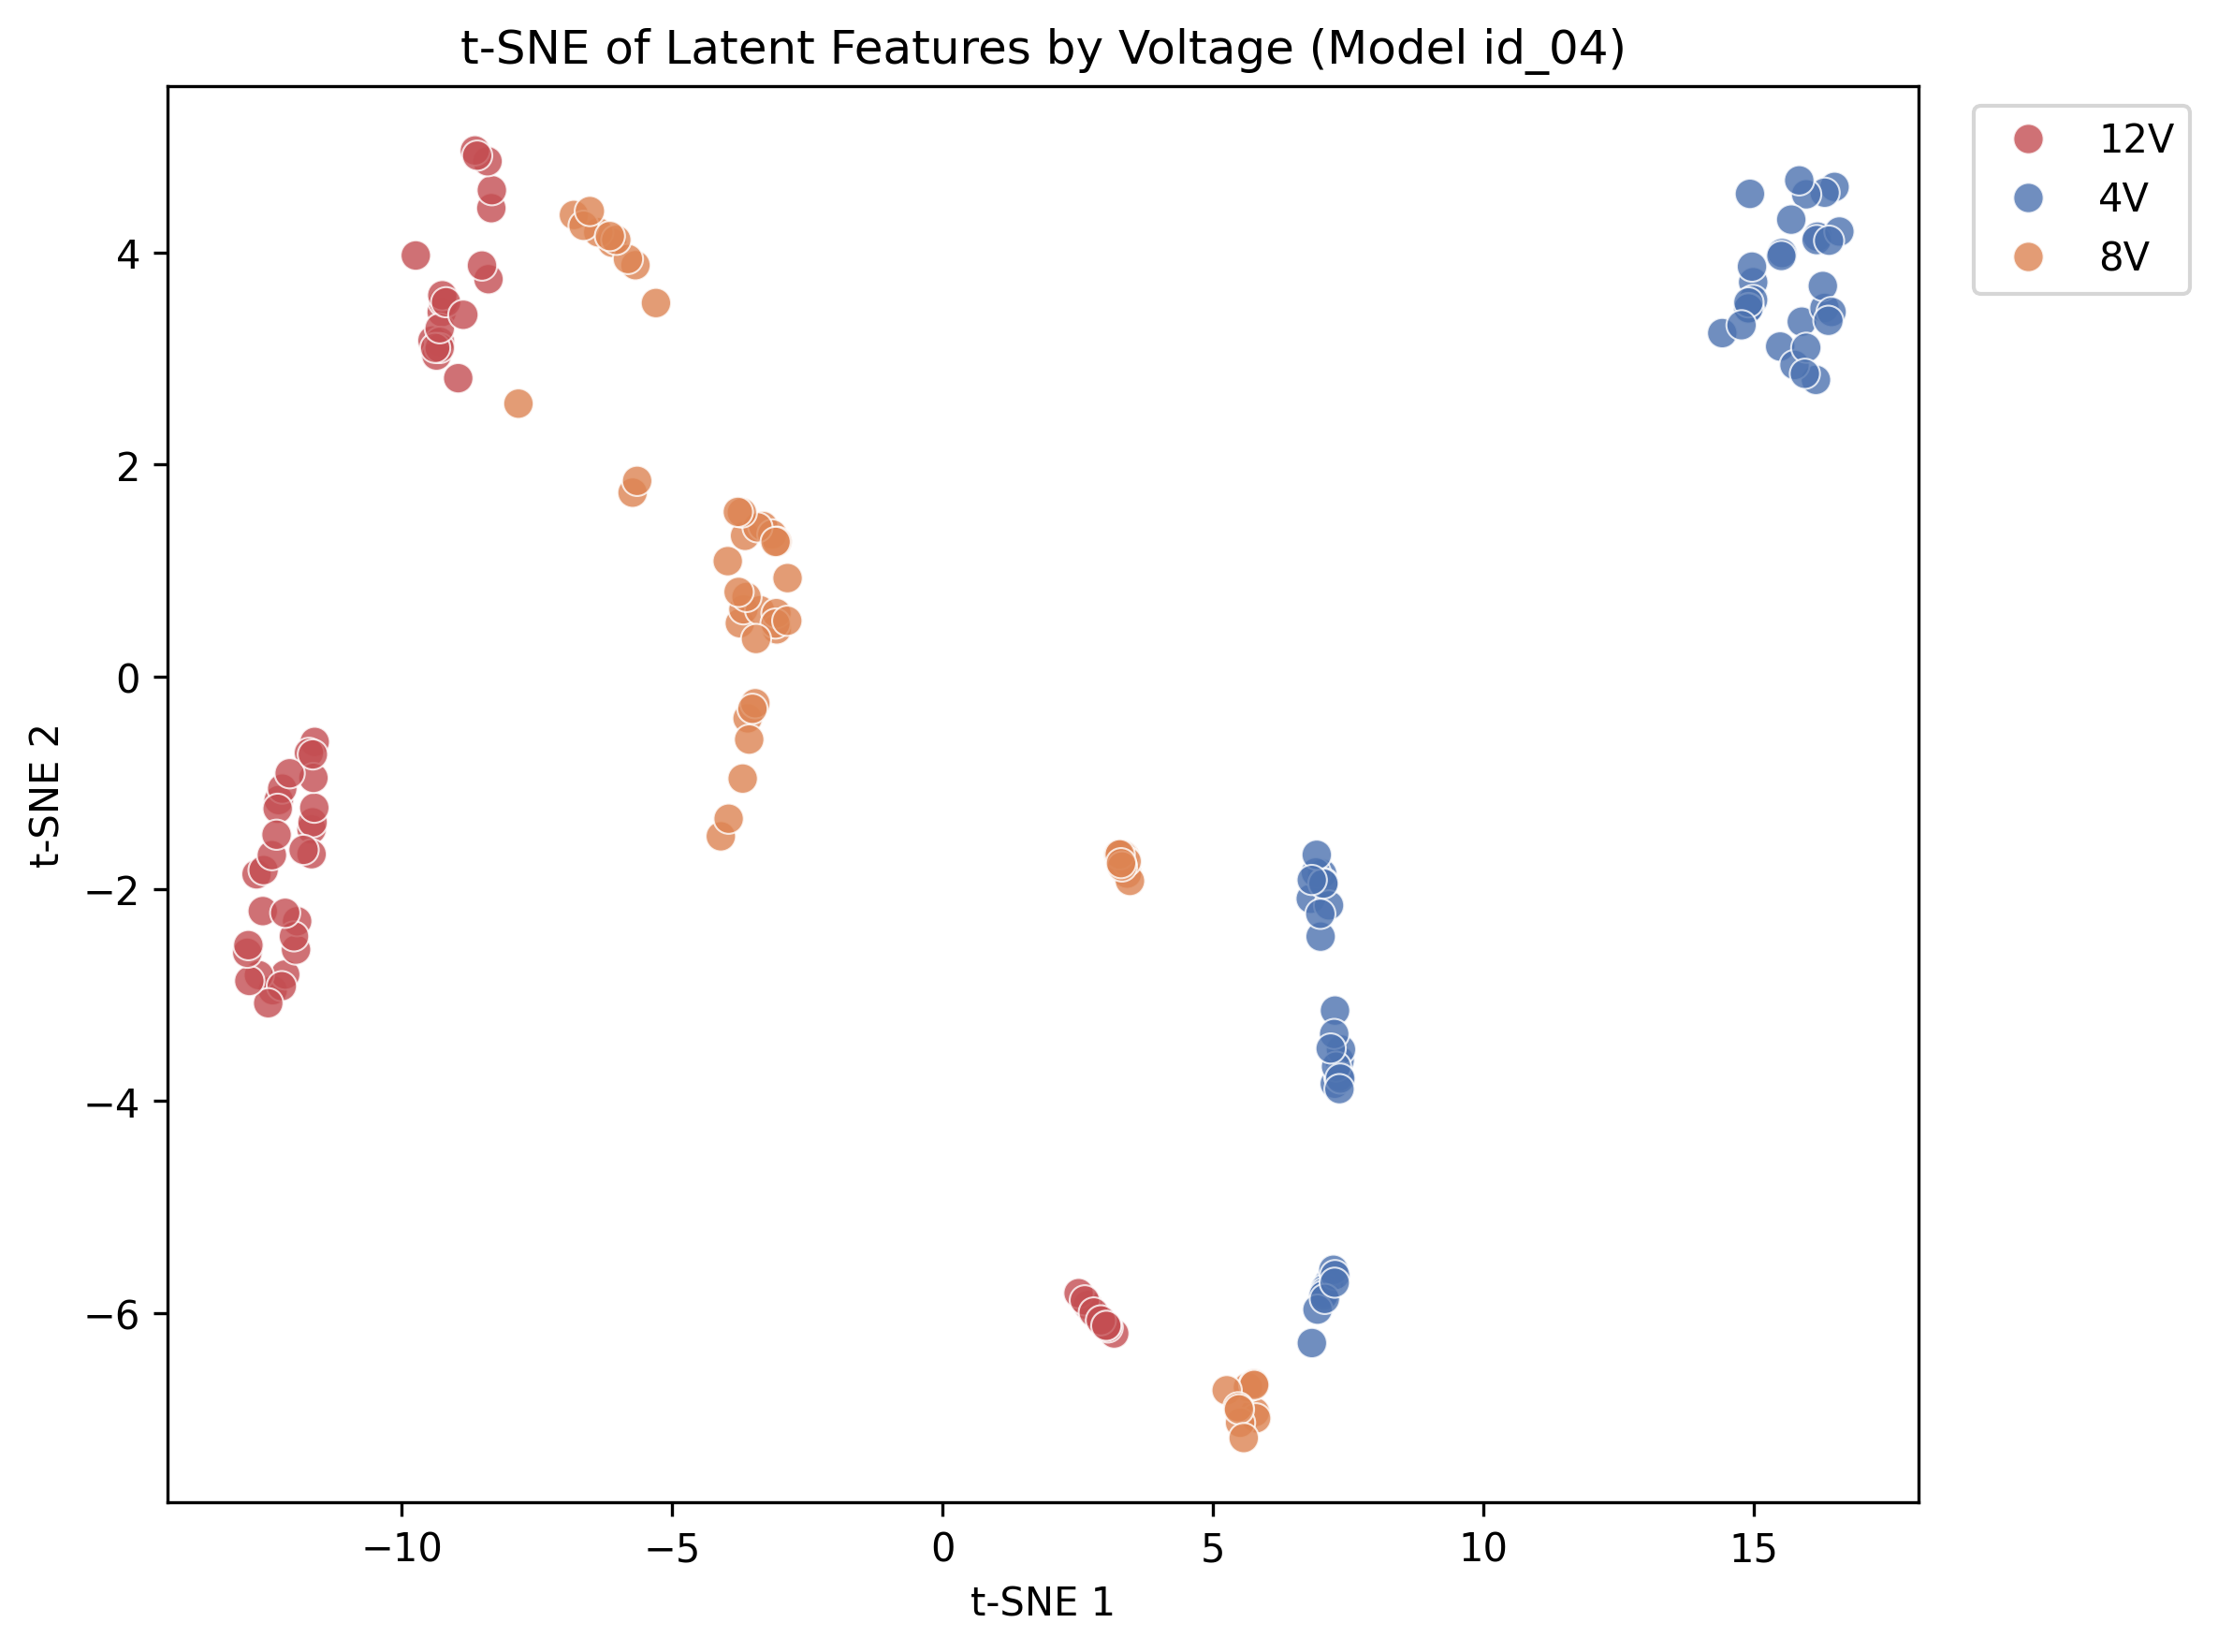
\includegraphics[width=0.75\textwidth]{figures/tsne_by_voltage_id_04.png}
    \caption{t-SNE visualization colored by voltage level. Sub-clusters within each condition correspond to different voltage levels, revealing a hierarchical structure: condition $\rightarrow$ voltage.}
    \label{fig:tsne-voltage}
\end{figure}

\paragraph{By noise environment.}
Fig.~\ref{fig:tsne-noise} shows that quiet and noise samples are largely intermixed within each cluster, rather than forming separate sub-groups. This suggests that the latent representation is \textbf{relatively robust to background noise variation}, which is a desirable property for practical deployment.

\begin{figure}[htbp]
    \centering
    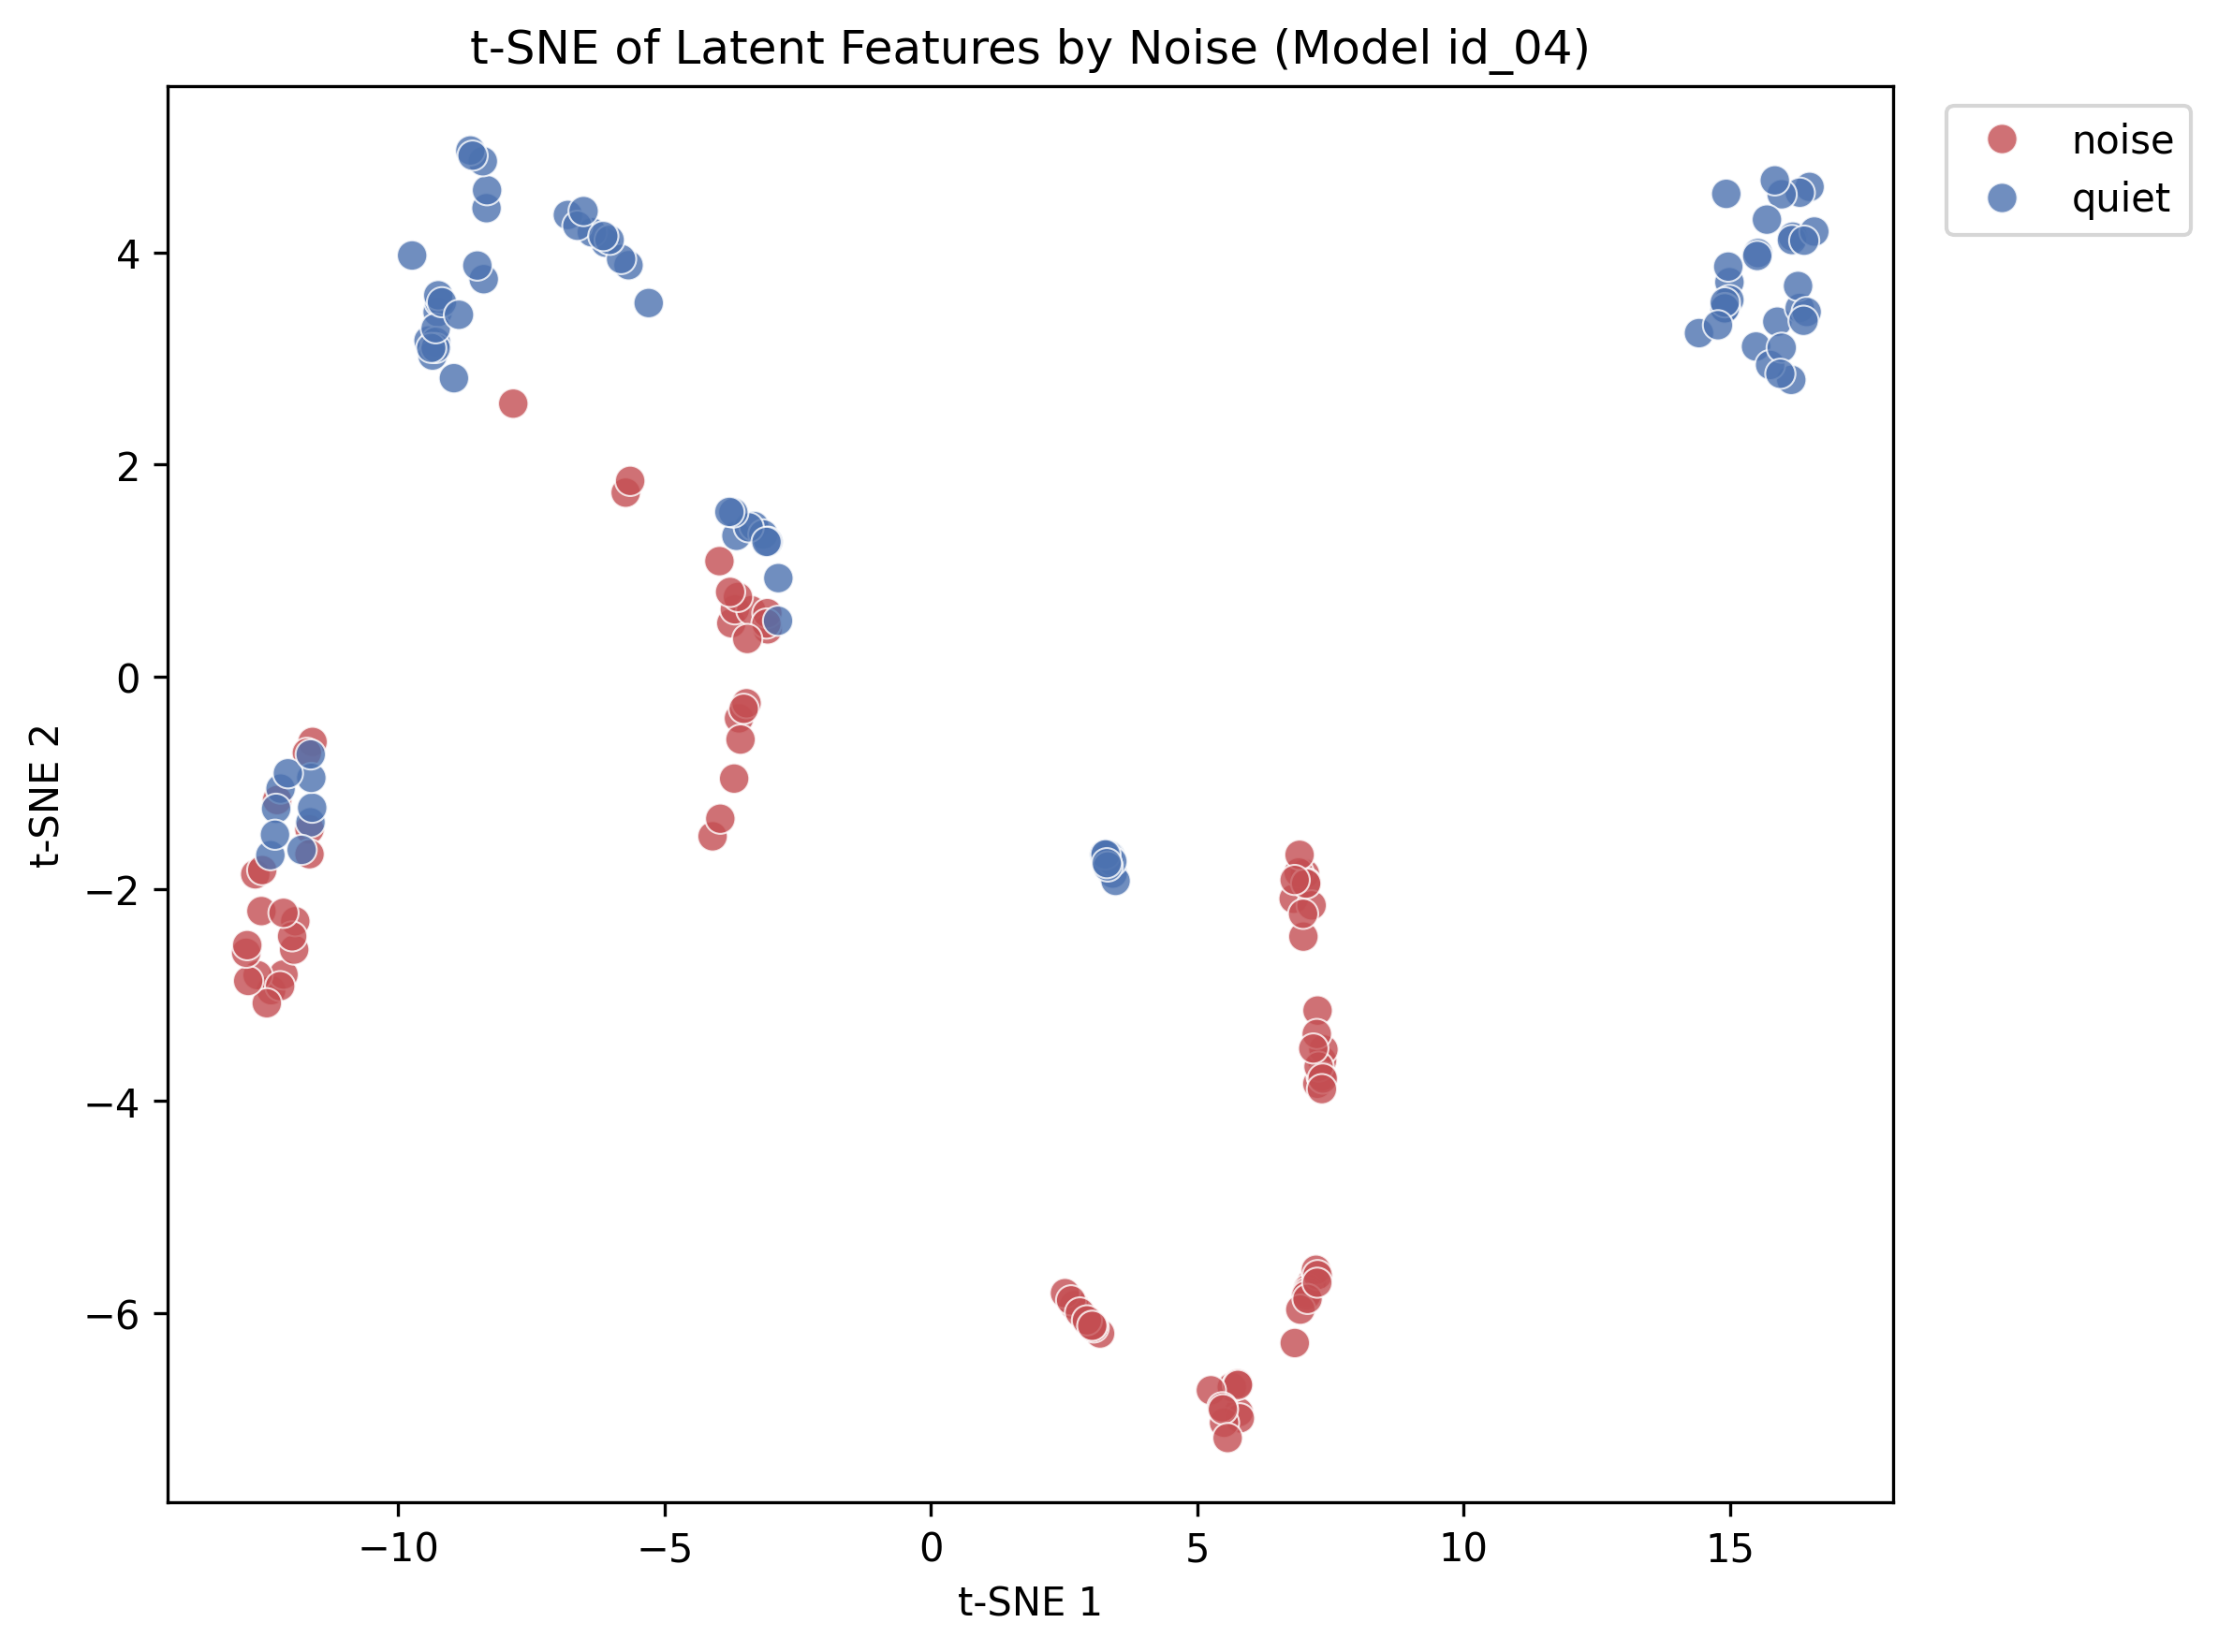
\includegraphics[width=0.75\textwidth]{figures/tsne_by_noise_id_04.png}
    \caption{t-SNE visualization colored by noise environment. Quiet and noise samples are well-mixed within clusters, indicating noise-invariant latent representations.}
    \label{fig:tsne-noise}
\end{figure}

\subsubsection{Multi-Class Classification}

To quantify the discriminative power of the latent features, we train three classifiers on the 8-dimensional latent mean vectors with 3-class labels (normal, blocked, imbalance). All classifiers use 5-fold stratified cross-validation with standardized features.

Table~\ref{tab:classification} summarizes the results.

\begin{table}[htbp]
\centering
\caption{Multi-class classification results on 8-dim latent features (5-fold stratified CV). Best results in \textbf{bold}.}
\label{tab:classification}
\begin{tabular}{lcccc}
\toprule
Classifier & Accuracy & F1 (macro) & Precision (macro) & Recall (macro) \\
\midrule
SVM (RBF)           & $0.722 \pm 0.077$ & $0.729 \pm 0.075$ & 0.784 & 0.722 \\
\textbf{Random Forest}       & $\mathbf{0.950 \pm 0.041}$ & $\mathbf{0.950 \pm 0.041}$ & \textbf{0.954} & \textbf{0.950} \\
KNN ($k$=5)         & $0.894 \pm 0.044$ & $0.891 \pm 0.045$ & 0.904 & 0.894 \\
\bottomrule
\end{tabular}
\end{table}

\textbf{Random Forest achieves 95.0\% accuracy} with a standard deviation of only 4.1\%, demonstrating that the pretrained latent features --- without any fine-tuning on our target domain --- already support highly accurate three-class discrimination. KNN ($k$=5) performs second-best at 89.4\%, while SVM (RBF) lags at 72.2\%.

The relatively low SVM performance is likely attributable to the activation structure: with only 2 out of 8 dimensions active and large-scale values ($z_0 \sim 150$, $z_7 \sim 160$), the RBF kernel's distance metric is dominated by these two dimensions, and the default hyperparameters may not be optimal. Random Forest, being invariant to monotonic feature transformations, naturally handles this without hyperparameter tuning.

Fig.~\ref{fig:confusion-matrix} shows the confusion matrix for the best classifier (Random Forest) refit on all data. While this is not a generalization estimate (the CV results in Table~\ref{tab:classification} serve that purpose), it confirms that the model correctly assigns all 180 samples with no confusion between any pair of conditions.

\begin{figure}[htbp]
    \centering
    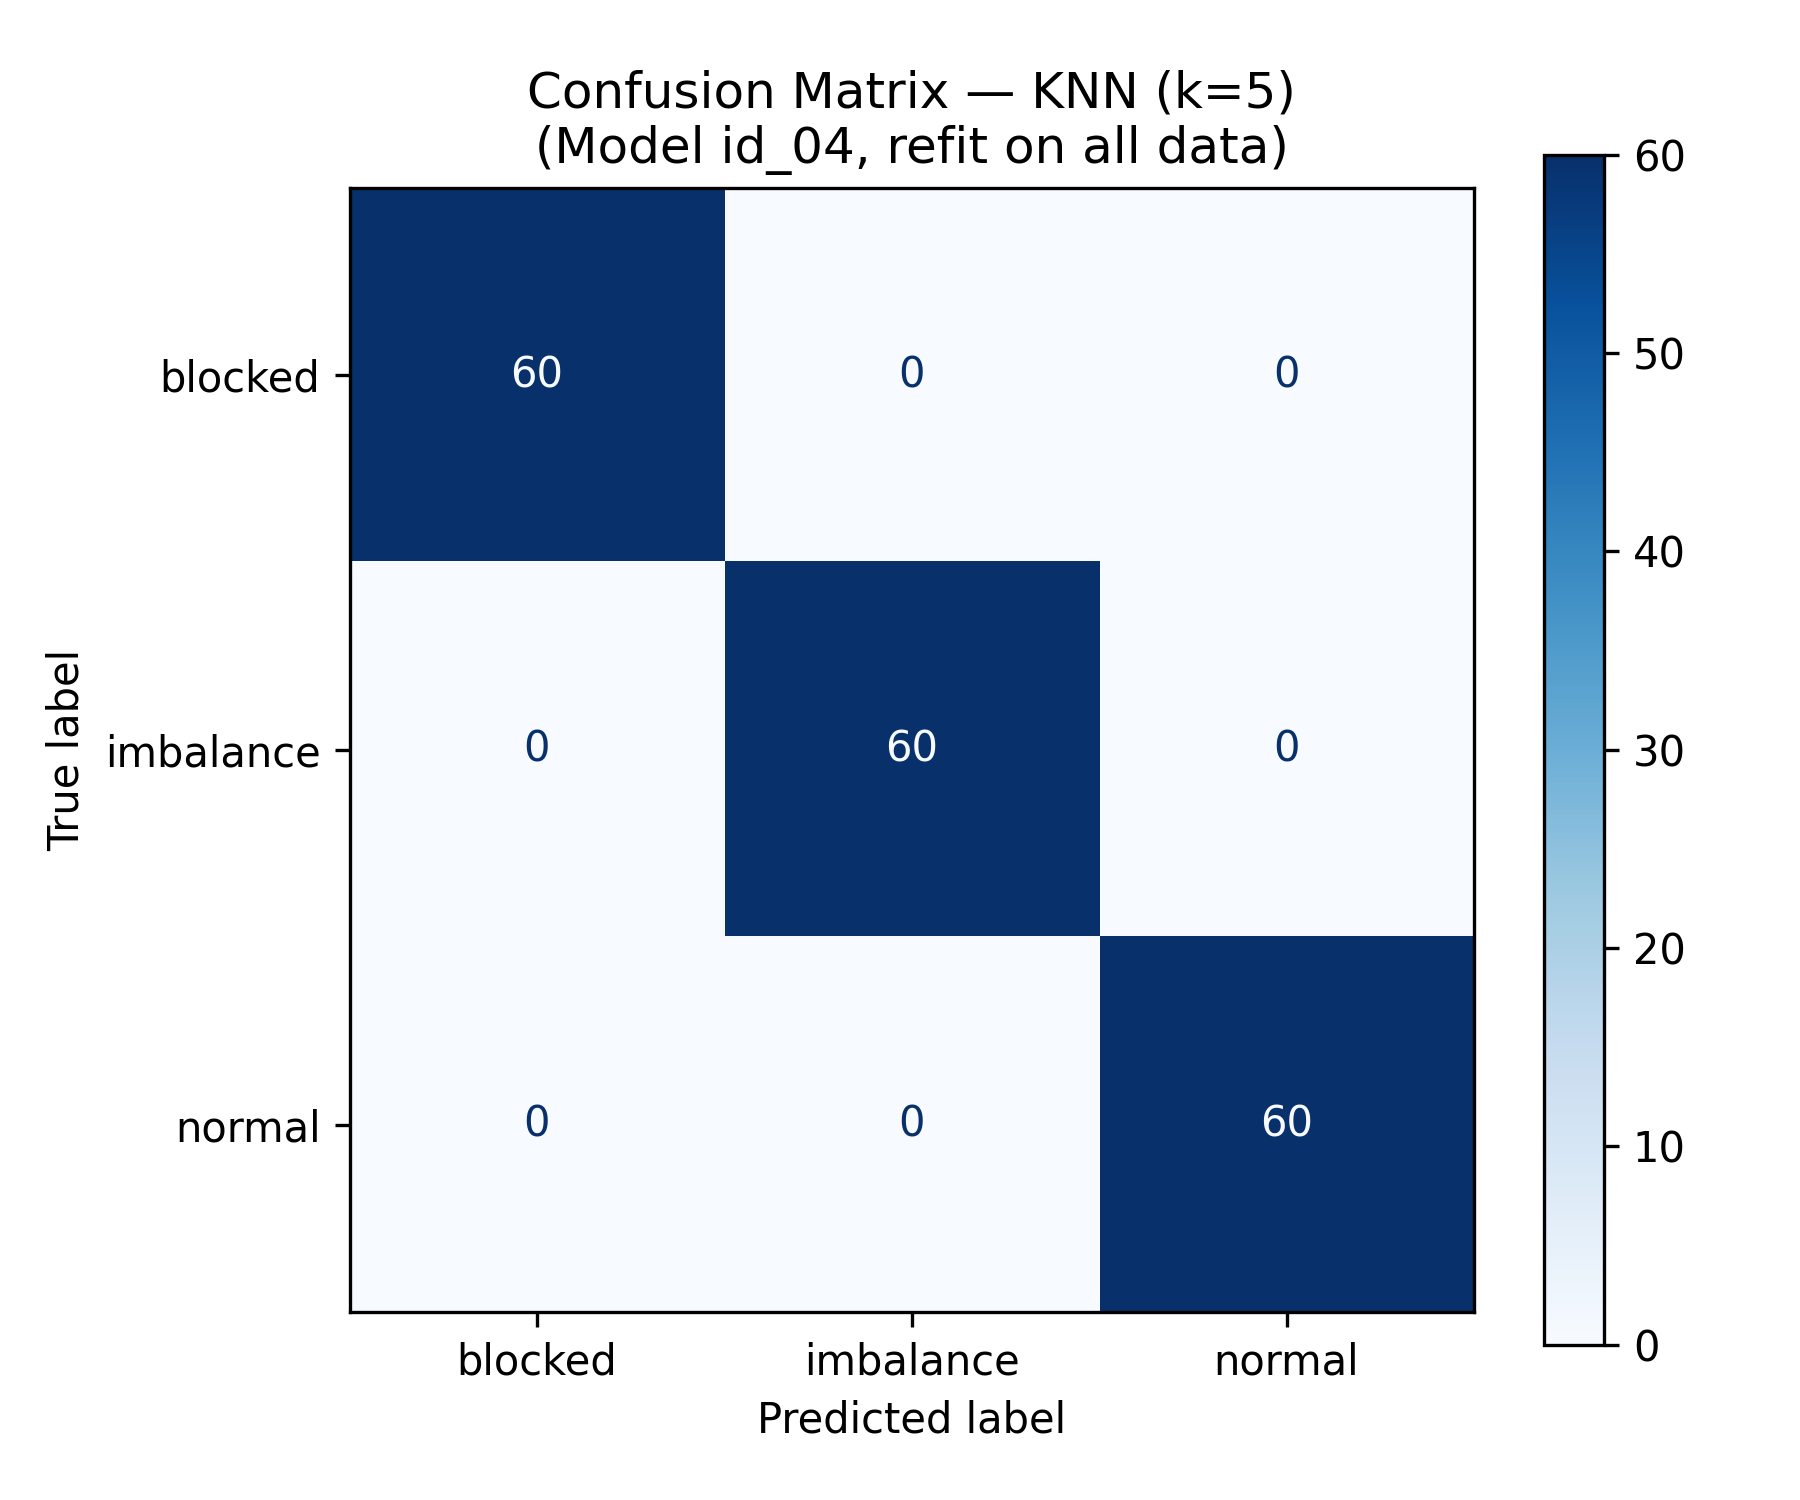
\includegraphics[width=0.5\textwidth]{figures/confusion_matrix_id_04.png}
    \caption{Confusion matrix for the Random Forest classifier refit on all 180 samples. Note: this is for visualization only; generalization performance is reported via 5-fold CV in Table~\ref{tab:classification}.}
    \label{fig:confusion-matrix}
\end{figure}

\subsubsection{Latent Analysis Summary}

The latent feature analysis yields four important findings:
\begin{enumerate}
    \item \textbf{The pretrained bottleneck encodes condition-discriminative information}: Despite being trained only on normal fan data from the MIMII source domain, the encoder's latent space separates three conditions with 95\% cross-validated accuracy.
    \item \textbf{Only 2 of 8 latent dimensions are active}: Dimensions $z_1$--$z_6$ are dead (zero-valued), meaning the effective latent dimensionality is 2. This suggests substantial capacity headroom for fine-tuning.
    \item \textbf{Latent representations encode a hierarchical structure}: The t-SNE analysis reveals a two-level organization --- condition at the coarse level and voltage at the fine level. Background noise does not form a significant axis of variation, indicating noise robustness.
    \item \textbf{Multi-class classification is feasible without retraining}: The Random Forest baseline (95.0\% CV accuracy) establishes a strong reference point for subsequent fine-tuning experiments.
\end{enumerate}


% --------------------------------------------------------
% 4.4 Fine-Tuning with Architecture Modification
% --------------------------------------------------------
\subsection{Fine-Tuning with Architecture Modification}
\label{sec:finetune}

The latent analysis in Section~\ref{sec:latent-analysis} revealed that 6 of 8 bottleneck dimensions are dead due to ReLU activation. In this section, we address both the dead-neuron problem and the domain shift simultaneously by (1) replacing the bottleneck ReLU with LeakyReLU and (2) fine-tuning the autoencoder on our target-domain normal data.

\subsubsection{Architecture Modification}

The only structural change is at the encoder's final activation:

\begin{table}[htbp]
\centering
\caption{Architecture comparison: baseline vs.\ fine-tuned model. The only change is the bottleneck activation function.}
\label{tab:arch-comparison}
\begin{tabular}{lll}
\toprule
Layer & Baseline & Fine-tuned \\
\midrule
Encoder: Linear(320, 64) + ReLU & \checkmark & \checkmark \\
Encoder: Linear(64, 64) + ReLU & \checkmark & \checkmark \\
Encoder: Linear(64, 8) + \textbf{ReLU} & \checkmark & $\rightarrow$ \textbf{LeakyReLU}($\alpha$=0.01) \\
\midrule
Decoder: Linear(8, 64) + ReLU & \checkmark & \checkmark \\
Decoder: Linear(64, 64) + ReLU & \checkmark & \checkmark \\
Decoder: Linear(64, 320) & \checkmark & \checkmark \\
\bottomrule
\end{tabular}
\end{table}

LeakyReLU replaces the hard zero-clipping of ReLU with a small negative slope ($\alpha = 0.01$), allowing gradients to flow through previously dead neurons during fine-tuning:
\begin{equation}
    \text{LeakyReLU}(x) = \begin{cases} x & \text{if } x \geq 0 \\ \alpha x & \text{if } x < 0 \end{cases}
\end{equation}

Since activation functions have no learnable parameters, the pretrained \texttt{id\_04} weights can be directly loaded into the new architecture without any adaptation.

\subsubsection{Fine-Tuning Protocol}

We fine-tune using only the 60 normal-condition samples, preserving the unsupervised anomaly detection paradigm:

\begin{itemize}
    \item \textbf{Training set}: 48 normal files ($\sim$14,400 frame-level vectors), randomly selected.
    \item \textbf{Validation set}: 12 normal files ($\sim$3,600 frame-level vectors), held out for early stopping.
    \item \textbf{Test set}: All 180 files (60 normal + 120 abnormal), used only for final evaluation.
    \item \textbf{Loss function}: MSE reconstruction loss (identical to original MIMII training).
    \item \textbf{Optimizer}: Adam, learning rate $10^{-4}$.
    \item \textbf{Early stopping}: Patience of 15 epochs on validation loss.
    \item \textbf{Epochs}: Up to 100 (ran full 100 without triggering early stopping).
\end{itemize}

Note that blocked and imbalance samples are \emph{never} seen during training. The model learns only what our fan sounds like under normal operation, and anomaly detection relies entirely on reconstruction error at test time.

\subsubsection{Training Dynamics}

Fig.~\ref{fig:training-curves} shows the training and validation loss curves. Both curves decrease smoothly and converge to approximately 5--6 MSE, with no divergence between training and validation loss, indicating that the model is not overfitting despite the small training set size.

\begin{figure}[htbp]
    \centering
    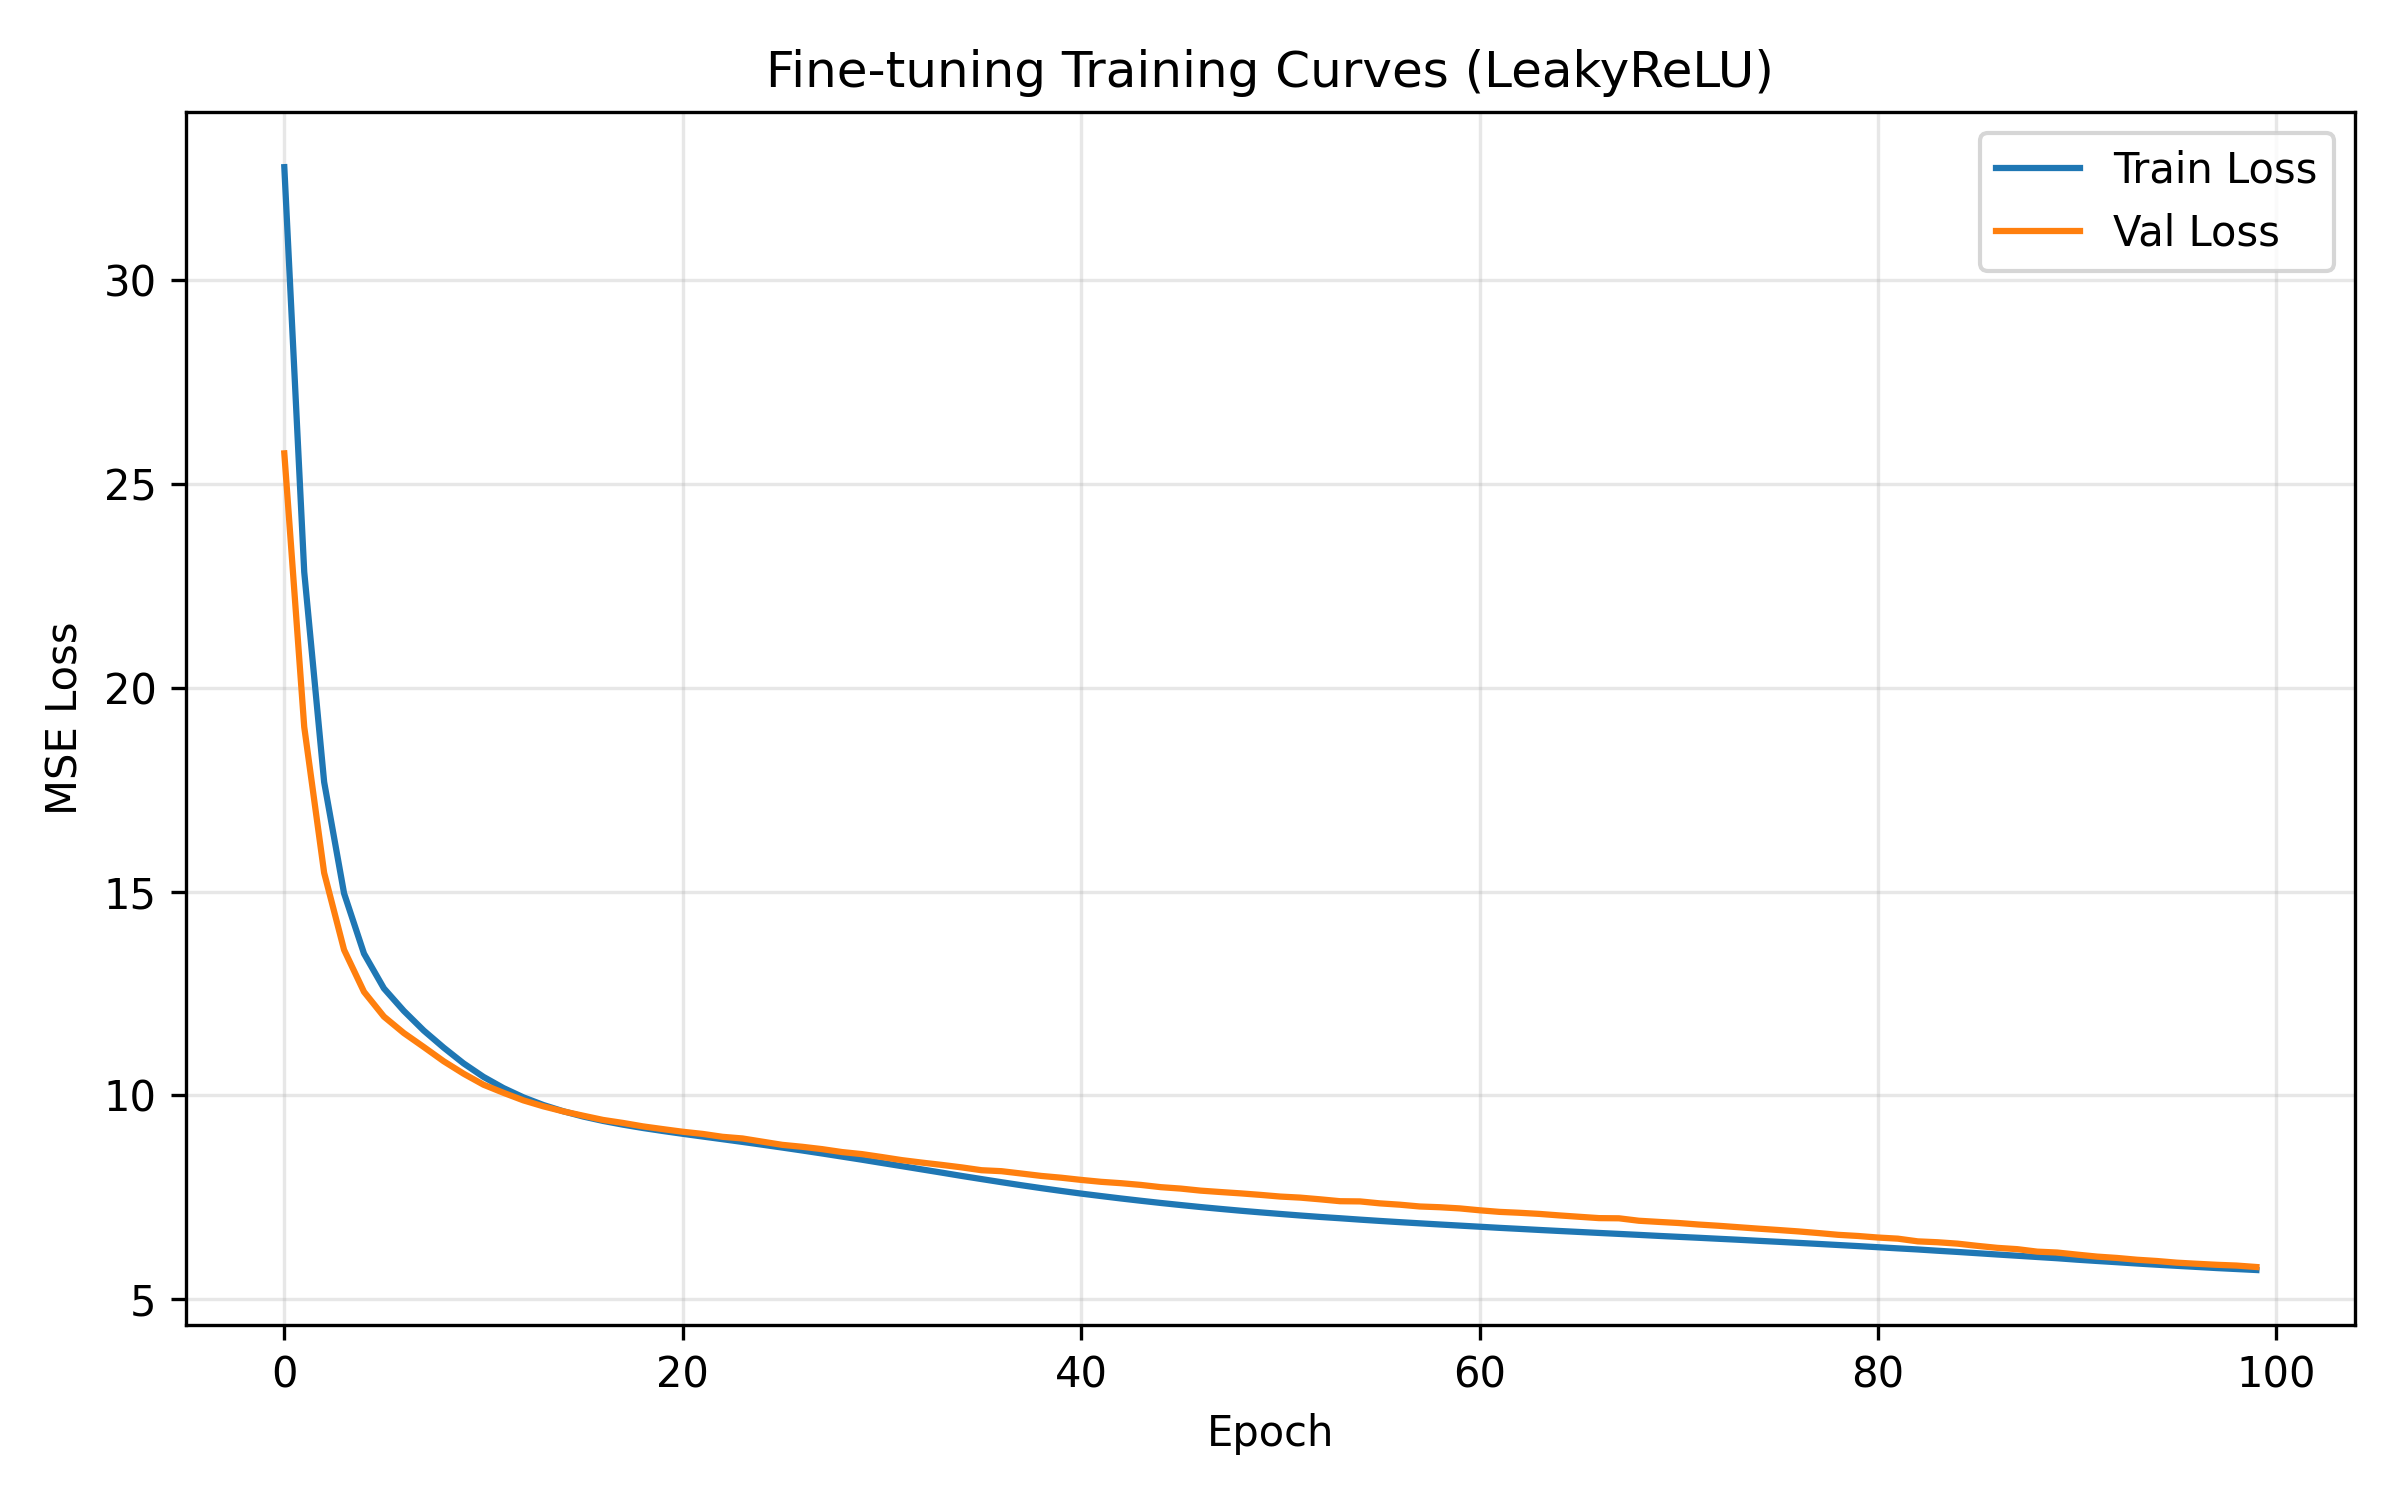
\includegraphics[width=0.7\textwidth]{figures/training_curves_finetuned.png}
    \caption{Fine-tuning training curves. Train and validation loss converge smoothly without overfitting.}
    \label{fig:training-curves}
\end{figure}

\subsubsection{Anomaly Detection Performance}

Table~\ref{tab:finetune-comparison} compares the anomaly detection performance before and after fine-tuning.

\begin{table}[htbp]
\centering
\caption{Binary anomaly detection: frozen baseline vs.\ fine-tuned model. All metrics are computed on the full 180-sample dataset with the best F1-maximizing threshold.}
\label{tab:finetune-comparison}
\begin{tabular}{lccc}
\toprule
Metric & Baseline (frozen ReLU) & Fine-tuned (LeakyReLU) & Change \\
\midrule
AUC                & 0.7693 & \textbf{0.9971} & +0.228 \\
Best F1            & 0.8458 & \textbf{0.9835} & +0.138 \\
Best Threshold     & 38.18  & \textbf{7.56}   & --- \\
Accuracy           & 0.7833 & \textbf{0.9722} & +0.189 \\
Precision          & 0.8045 & \textbf{0.9756} & +0.171 \\
Recall             & 0.8917 & \textbf{0.9917} & +0.100 \\
\bottomrule
\end{tabular}
\end{table}

The results show dramatic improvements:

\begin{itemize}
    \item \textbf{AUC improves from 0.769 to 0.997} (+0.228), indicating near-perfect ranking of normal vs.\ abnormal samples. The model now assigns higher MSE to virtually every abnormal file than to every normal file.
    \item \textbf{F1 improves from 0.846 to 0.984} (+0.138), with both precision and recall exceeding 0.97.
    \item \textbf{The optimal threshold drops from 38.18 to 7.56}, returning to the same scale as the source-domain thresholds (5--7). This is direct evidence that fine-tuning has successfully eliminated the domain shift in reconstruction error magnitude: the model now reconstructs our normal fan sounds with similarly low error as it did for its original MIMII training data.
\end{itemize}

\subsubsection{Latent Dimension Activation}

Fig.~\ref{fig:latent-dims-ft} shows the per-dimension boxplot after fine-tuning.

\begin{figure}[htbp]
    \centering
    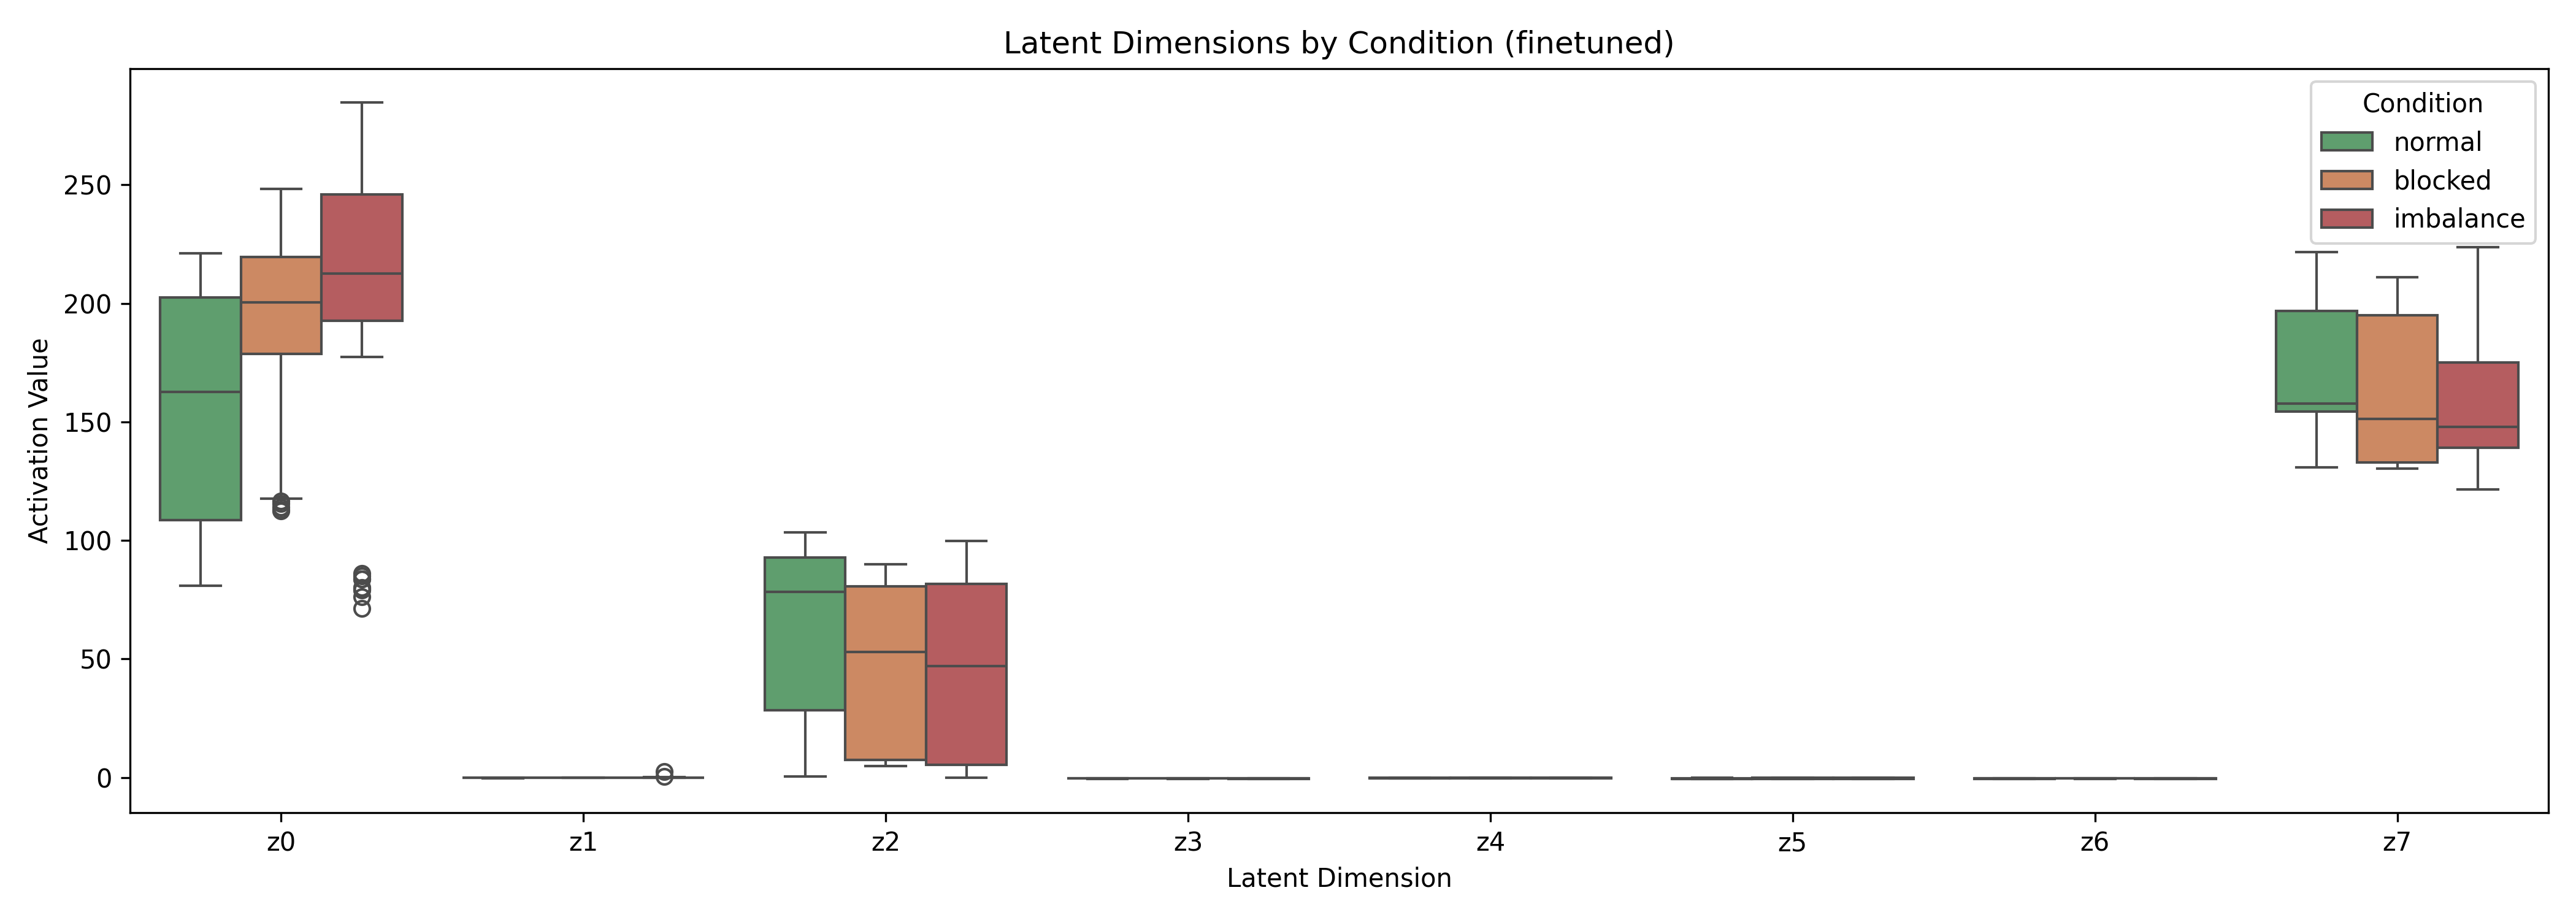
\includegraphics[width=\textwidth]{figures/latent_dimensions_by_condition_finetuned.png}
    \caption{Latent dimension activations after fine-tuning with LeakyReLU. Compared to Fig.~\ref{fig:latent-dims}, dimension $z_2$ is now active, and $z_1$ shows emerging activity.}
    \label{fig:latent-dims-ft}
\end{figure}

\begin{table}[htbp]
\centering
\caption{Per-dimension activation status before and after fine-tuning.}
\label{tab:dim-activation}
\begin{tabular}{lccl}
\toprule
Dimension & Baseline (frozen) & Fine-tuned & Change \\
\midrule
$z_0$ & ACTIVE ($\sim$100--200) & ACTIVE ($\sim$110--250) & Range expanded \\
$z_1$ & DEAD (0.0) & Emerging ($\sim$0--80 outliers) & Partially awakened \\
$z_2$ & DEAD (0.0) & \textbf{ACTIVE ($\sim$5--90)} & \textbf{Fully activated} \\
$z_3$--$z_6$ & DEAD (0.0) & Near-zero ($< 1.0$) & Minimal change \\
$z_7$ & ACTIVE ($\sim$120--210) & ACTIVE ($\sim$130--195) & Stable \\
\bottomrule
\end{tabular}
\end{table}

The number of active dimensions increased from 2 to 4 (counting $z_1$'s emerging activity). Notably, the newly activated $z_2$ shows clear condition-dependent variation: normal samples have higher $z_2$ values ($\sim$60--90) than blocked ($\sim$40--70) and imbalance ($\sim$30--60) samples, providing additional discriminative information. The remaining dimensions ($z_3$--$z_6$) show small negative values enabled by LeakyReLU but not yet meaningful variation --- they may require longer training, more data, or further architectural changes to fully activate.

\subsubsection{t-SNE Visualization After Fine-Tuning}

Figs.~\ref{fig:tsne-condition-ft} and~\ref{fig:tsne-voltage-ft} show t-SNE embeddings of the fine-tuned latent features.

\begin{figure}[htbp]
    \centering
    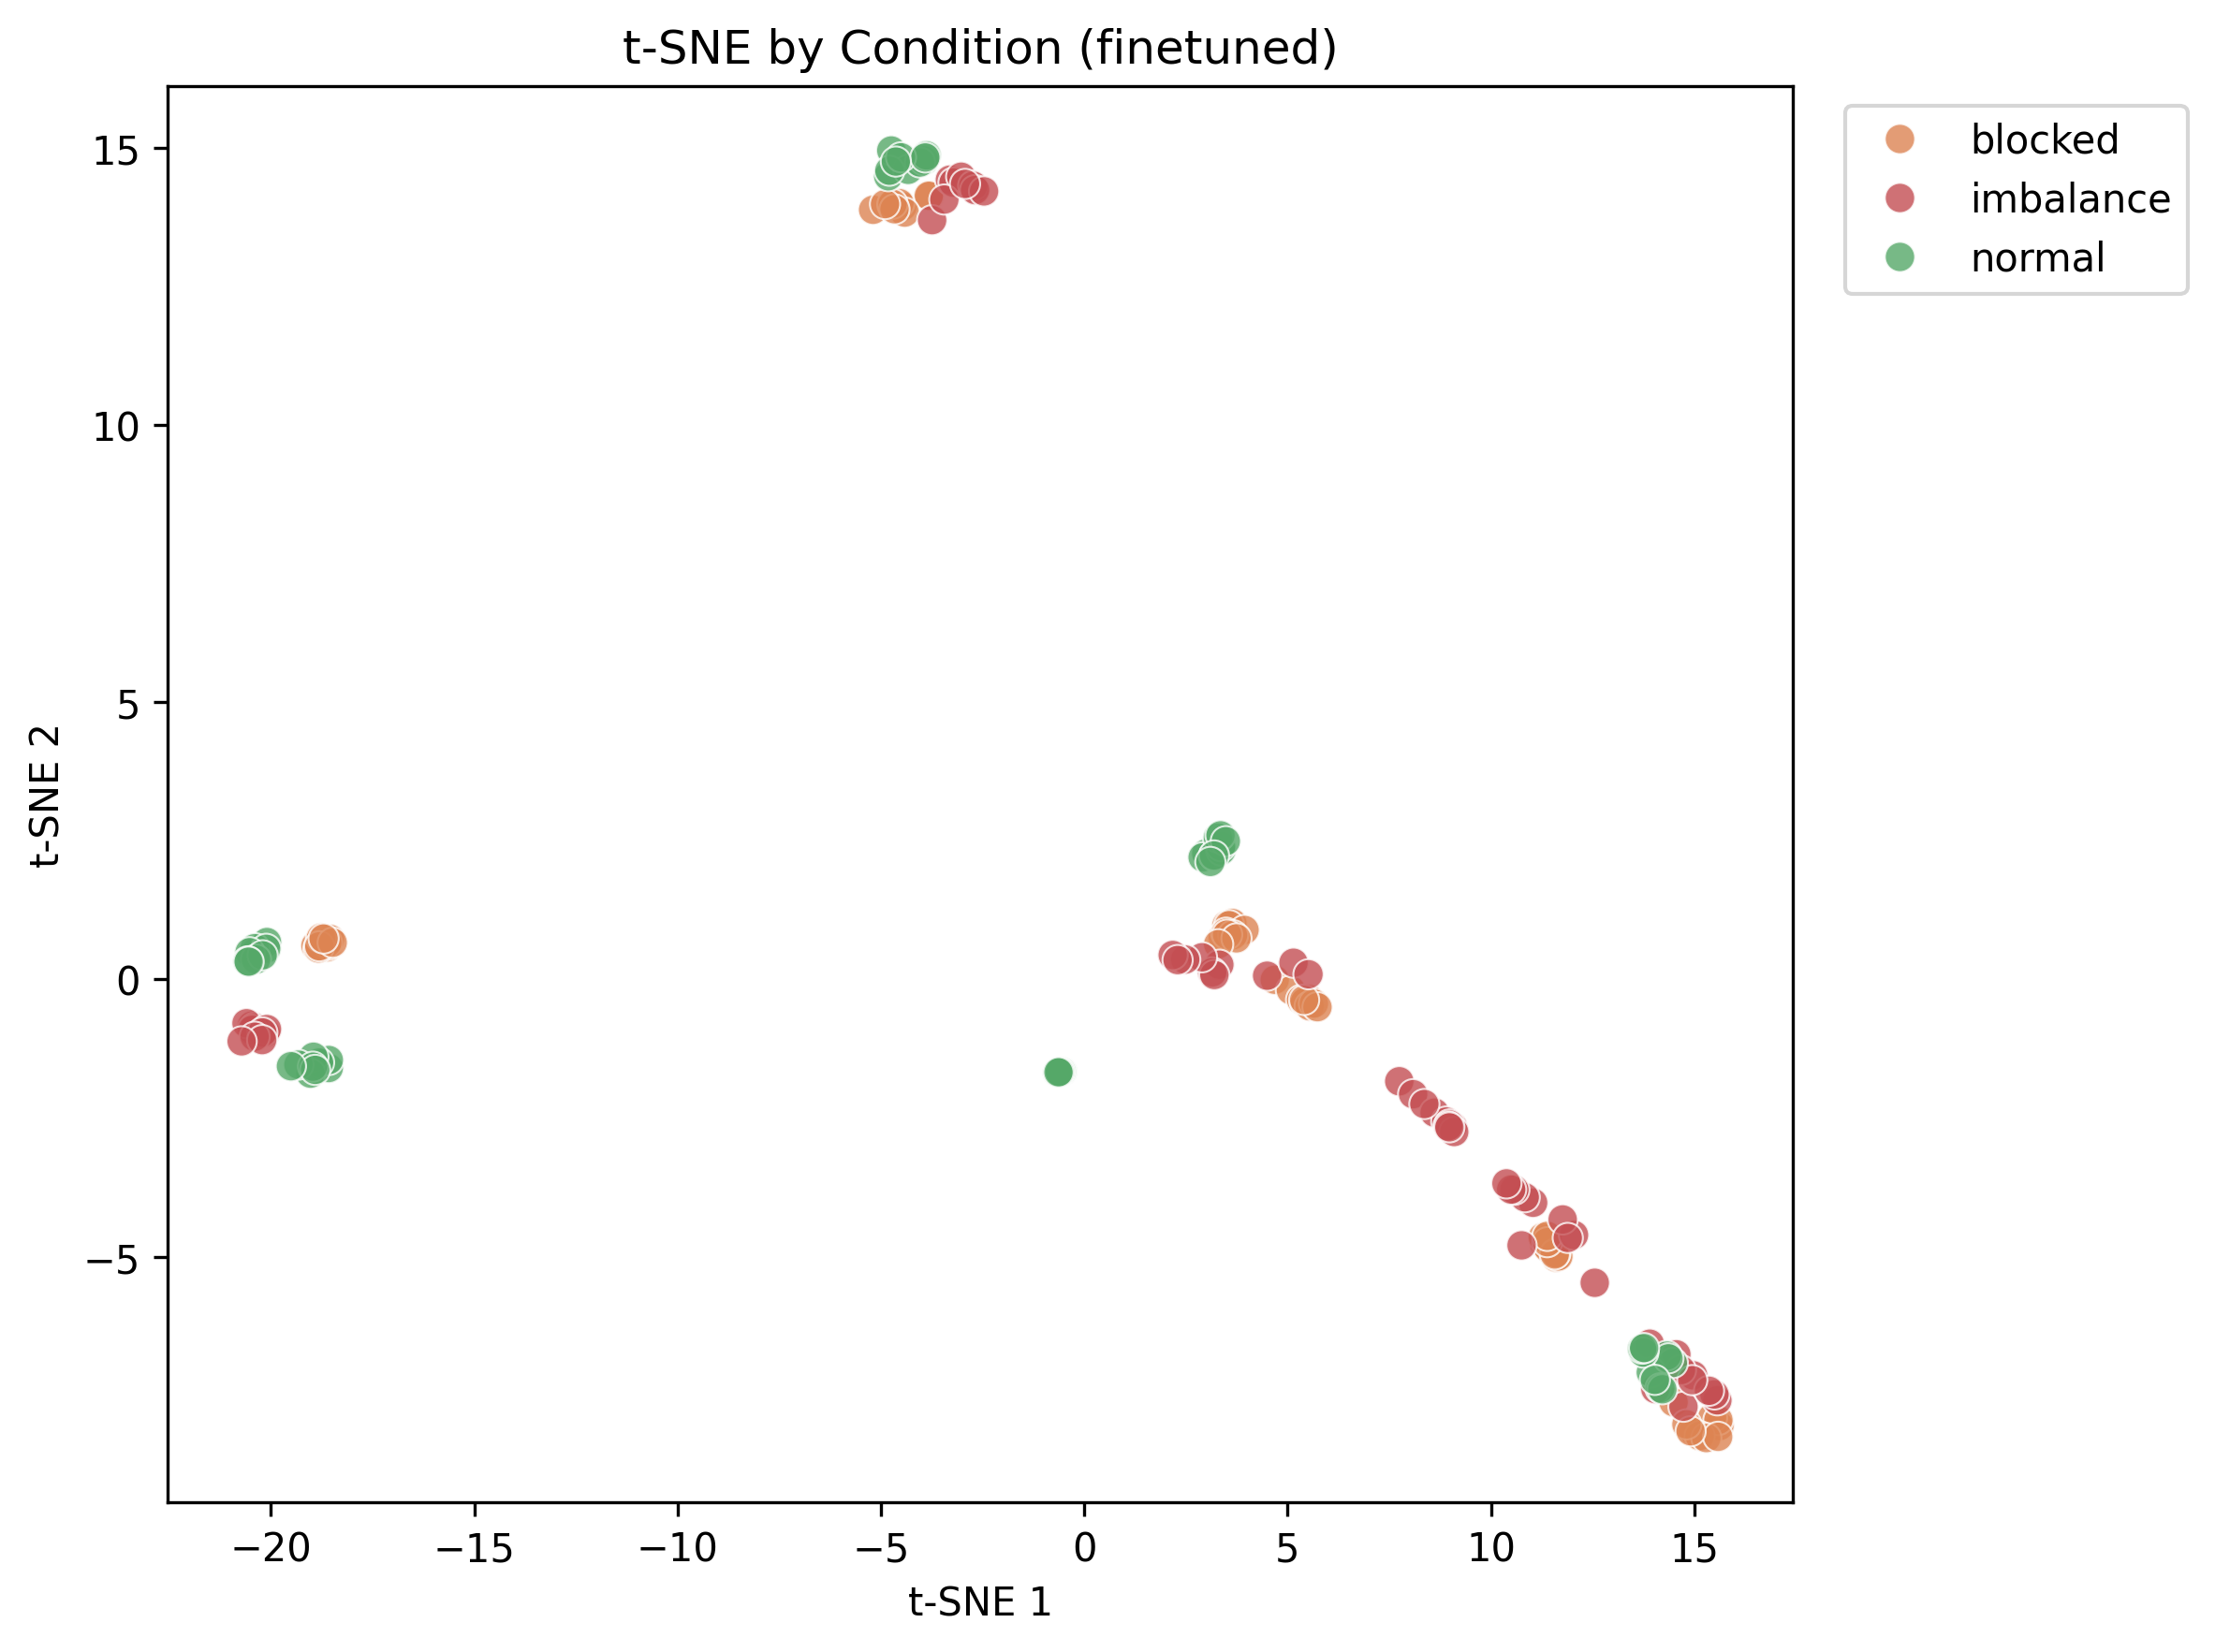
\includegraphics[width=0.75\textwidth]{figures/tsne_by_condition_finetuned.png}
    \caption{t-SNE of fine-tuned latent features by condition. Compared to Fig.~\ref{fig:tsne-condition}, clusters are more compact and inter-class gaps are wider.}
    \label{fig:tsne-condition-ft}
\end{figure}

\begin{figure}[htbp]
    \centering
    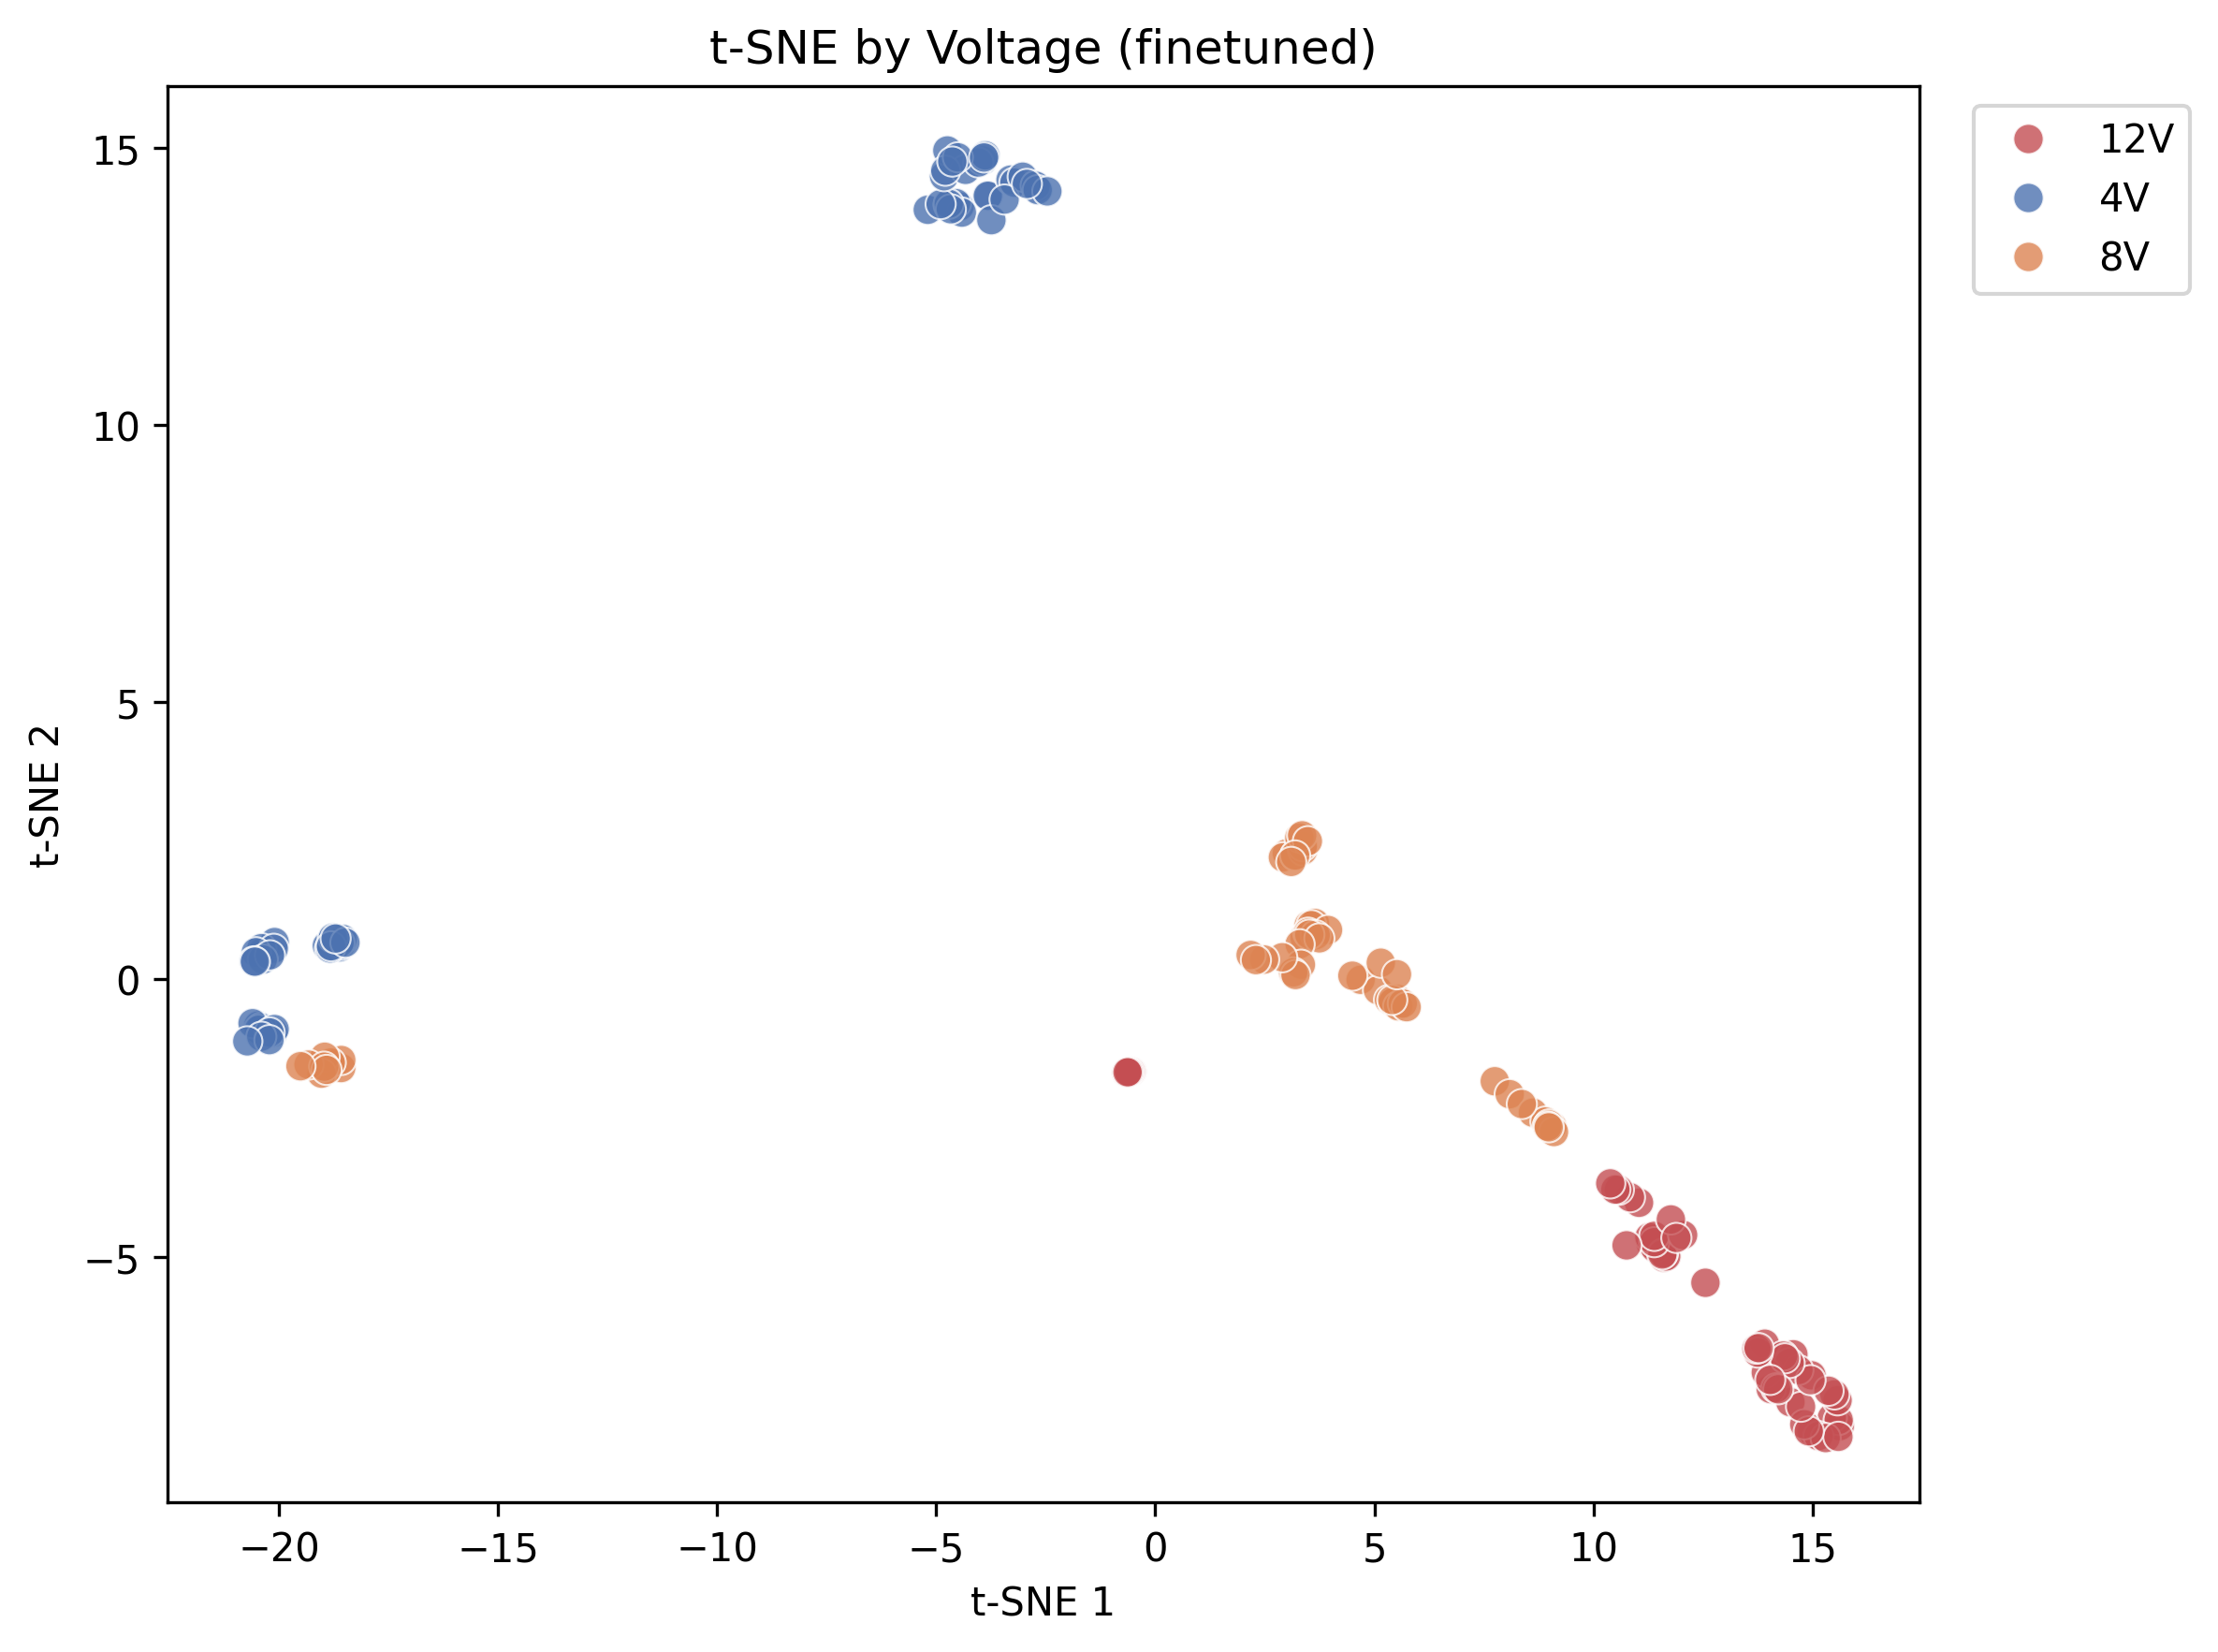
\includegraphics[width=0.75\textwidth]{figures/tsne_by_voltage_finetuned.png}
    \caption{t-SNE of fine-tuned latent features by voltage. The hierarchical structure (condition $\rightarrow$ voltage) is preserved and more clearly organized.}
    \label{fig:tsne-voltage-ft}
\end{figure}

Compared to the frozen-baseline t-SNE (Figs.~\ref{fig:tsne-condition}--\ref{fig:tsne-voltage}), the fine-tuned embeddings show tighter within-class clustering and larger inter-class margins. The voltage-level sub-structure is also more clearly organized, with 4V, 8V, and 12V forming a regular gradient within each condition cluster.

\subsubsection{Multi-Class Classification After Fine-Tuning}

Table~\ref{tab:classification-ft} compares classification results before and after fine-tuning.

\begin{table}[htbp]
\centering
\caption{Multi-class classification on latent features: frozen baseline vs.\ fine-tuned (5-fold stratified CV).}
\label{tab:classification-ft}
\begin{tabular}{l cc cc}
\toprule
 & \multicolumn{2}{c}{Accuracy} & \multicolumn{2}{c}{F1 (macro)} \\
\cmidrule(lr){2-3} \cmidrule(lr){4-5}
Classifier & Baseline & Fine-tuned & Baseline & Fine-tuned \\
\midrule
SVM (RBF)      & $0.722 \pm 0.077$ & $0.744 \pm 0.069$ & $0.729$ & $0.728$ \\
Random Forest  & $0.950 \pm 0.041$ & $0.950 \pm 0.037$ & $0.950$ & $0.950$ \\
KNN ($k$=5)    & $0.894 \pm 0.044$ & $0.928 \pm 0.028$ & $0.891$ & $0.927$ \\
\bottomrule
\end{tabular}
\end{table}

The three-class accuracy remains at 95.0\% for Random Forest, but two secondary improvements are noteworthy:
\begin{itemize}
    \item \textbf{KNN improved from 89.4\% to 92.8\%}: Since KNN directly reflects the geometric structure of the latent space, this improvement confirms that the fine-tuned representations have better local separability.
    \item \textbf{Standard deviation decreased} for all classifiers (e.g., RF: $0.041 \rightarrow 0.037$; KNN: $0.044 \rightarrow 0.028$), indicating more consistent performance across cross-validation folds.
\end{itemize}

The fact that RF accuracy did not increase beyond 95\% is expected: with only 180 samples, the 9 misclassified files likely represent genuinely ambiguous boundary cases (e.g., low-voltage blocked samples that sound similar to normal) that require either more training data or a supervised classification head to resolve.

\subsubsection{Fine-Tuning Summary}

The combined architecture modification (LeakyReLU) and target-domain fine-tuning yields substantial improvements:

\begin{enumerate}
    \item \textbf{Anomaly detection}: AUC $0.769 \rightarrow 0.997$, F1 $0.846 \rightarrow 0.984$. The fine-tuned model achieves near-perfect binary anomaly detection on our dataset.
    \item \textbf{Domain adaptation}: The optimal threshold returned from 38.18 to 7.56, matching the source-domain scale and confirming successful domain alignment.
    \item \textbf{Latent activation}: Active dimensions increased from 2/8 to 4/8, with $z_2$ newly contributing condition-discriminative information.
    \item \textbf{Representation quality}: t-SNE shows tighter clusters, and KNN accuracy improved from 89.4\% to 92.8\%, confirming better geometric structure in the latent space.
\end{enumerate}


% ############################################################
% Section 5: Future Work
% ############################################################
\section{Future Work}
\label{sec:future}

The fine-tuning experiment in Section~\ref{sec:finetune} demonstrated large gains in anomaly detection and partial activation of dead neurons. However, several directions remain open for further improvement.

\subsection{Stage 1 Improvements: Data and Architecture}

\subsubsection{Collecting More Experimental Data}

The current dataset contains only 180 samples (60 per condition). While sufficient for the present evaluation, this limited scale constrains both training and evaluation:

\begin{itemize}
    \item \textbf{More normal samples for fine-tuning}: The autoencoder was fine-tuned on only 48 normal files ($\sim$14,400 frame vectors). Increasing this to 200+ files would provide greater acoustic diversity (e.g., different ambient temperatures, time-of-day effects) and enable the model to learn a more robust representation of normal operation.
    \item \textbf{More anomaly variants}: Currently only two fault types (blocked, imbalance) are represented. Adding additional conditions such as bearing wear, loose mounting, or partial blade damage would test the model's ability to generalize to unseen anomaly types.
    \item \textbf{More fan units}: All recordings come from a single fan. Collecting data from multiple fan units of the same model (or different models) would enable cross-unit generalization experiments, directly paralleling the MIMII multi-ID setup.
    \item \textbf{Finer voltage granularity}: The current 4V/8V/12V levels provide coarse speed variation. Adding intermediate voltages (e.g., 6V, 10V) would yield a denser sampling of the operating-speed axis, enabling smoother interpolation in the latent space.
\end{itemize}

\subsubsection{Further Architecture Exploration}

The LeakyReLU modification activated 2 additional dimensions (from 2/8 to 4/8), but 4 dimensions remain inactive. Several further modifications could be explored:

\begin{itemize}
    \item \textbf{Bottleneck size sweep}: Systematically vary the bottleneck dimension (2, 4, 8, 16, 32) and compare both reconstruction quality and classification accuracy. The current 8-dim bottleneck may be either too large (leading to unused capacity) or too small (limiting representational power once more dimensions activate).
    \item \textbf{Deeper LeakyReLU application}: Apply LeakyReLU to \emph{all} layers (not just the bottleneck) to ensure gradient flow throughout the entire network during fine-tuning.
    \item \textbf{Batch normalization}: Insert BatchNorm layers before activations to stabilize the distribution of layer inputs. This may help activate the remaining dead dimensions by preventing extreme weight magnitudes.
    \item \textbf{Variational autoencoder (VAE)}: Replace the deterministic bottleneck with a stochastic $\mu + \sigma$ sampling layer. VAE training encourages a smooth, continuous latent space, which would naturally prevent dead dimensions and produce more interpretable latent representations. The VAE loss adds a KL divergence term:
    \begin{equation}
        \mathcal{L}_{\text{VAE}} = \mathcal{L}_{\text{MSE}} + \beta \cdot D_{\text{KL}}\big(q(\mathbf{z}|\mathbf{x}) \,\|\, p(\mathbf{z})\big)
    \end{equation}
    \item \textbf{Convolutional encoder}: Replace the fully-connected encoder with 1D or 2D convolutions operating directly on the mel spectrogram. This preserves local time-frequency structure that the frame-stacking approach may lose.
\end{itemize}

\subsection{Stage 2: Multi-Task Learning with Classification Head}
\label{sec:stage2}

The fine-tuned model from Stage~1 achieves 95\% three-class accuracy using an external Random Forest classifier on frozen latent features. Stage~2 aims to surpass this by training the encoder and a classification head jointly in an end-to-end manner.

\subsubsection{Architecture}

A linear classification head is attached to the bottleneck:

\begin{equation}
    \hat{y} = \text{softmax}\big(W_c \cdot \mathbf{z} + b_c\big), \quad W_c \in \mathbb{R}^{3 \times 8},\; b_c \in \mathbb{R}^3
\end{equation}

The model now has two output paths:

\begin{center}
\begin{tabular}{rcl}
Input(320) $\rightarrow$ Encoder $\rightarrow$ & Latent(8) & $\rightarrow$ Decoder $\rightarrow$ Reconstruction(320) \\
 & $\downarrow$ & \\
 & Classification Head & $\rightarrow$ Prediction(3 classes) \\
\end{tabular}
\end{center}

\subsubsection{Training Objective}

The combined loss balances reconstruction and classification:
\begin{equation}
    \mathcal{L} = \alpha \cdot \mathcal{L}_{\text{MSE}} + \beta \cdot \mathcal{L}_{\text{CE}}
\end{equation}
where $\mathcal{L}_{\text{MSE}}$ is the reconstruction loss (preserving anomaly detection capability), $\mathcal{L}_{\text{CE}}$ is the cross-entropy classification loss, and $\alpha, \beta$ are balancing coefficients. The reconstruction term acts as a regularizer, preventing the encoder from collapsing to a representation that is discriminative but not generalizable.

\subsubsection{Data Requirements and Paradigm Shift}

Unlike Stage~1 (unsupervised, normal-only training), Stage~2 requires \textbf{labeled data from all three conditions}. This fundamentally shifts the paradigm from unsupervised anomaly detection to supervised multi-class classification. The data split would be:

\begin{itemize}
    \item \textbf{Training}: 144 files (48 per condition), using all three labels.
    \item \textbf{Testing}: 36 files (12 per condition), evaluated via 5-fold CV for stability.
\end{itemize}

The 95\% RF accuracy from Stage~1 serves as the baseline that Stage~2 must exceed to justify the added complexity.

\subsubsection{Expected Outcomes}

\begin{itemize}
    \item End-to-end gradient flow from the classification loss back through the encoder should activate more latent dimensions by creating explicit pressure to separate the three classes.
    \item The reconstruction loss term prevents the encoder from overfitting to the classification task, maintaining its ability to detect \emph{unseen} anomaly types that were not present in training.
    \item If successful, the same model could serve dual purposes: binary anomaly detection (via MSE thresholding) and multi-class fault diagnosis (via the classification head).
\end{itemize}

\subsection{Extended Evaluation}

Regardless of the model architecture, the following evaluation extensions are planned:
\begin{itemize}
    \item \textbf{Leave-one-voltage-out cross-validation}: Train on two voltage levels and test on the third to assess generalization across operating speeds.
    \item \textbf{Per-condition AUC analysis}: Compute normal-vs-blocked and normal-vs-imbalance AUC separately to identify which fault type is harder to detect.
    \item \textbf{Feature importance analysis}: Use Random Forest feature importances or SHAP values to identify which latent dimensions contribute most to classification decisions.
    \item \textbf{Real-time deployment feasibility}: Profile the inference latency of the fine-tuned model to assess whether real-time monitoring is practical on edge devices.
\end{itemize}


% ############################################################
% Section 6: Conclusion
% ############################################################
\section{Conclusion}
\label{sec:conclusion}

This report presents a systematic study on acoustic anomaly detection for HVAC fan systems, progressing from cross-domain transfer evaluation through latent space analysis to architecture modification and fine-tuning. Our key contributions and findings are:

\begin{enumerate}
    \item We collected a controlled 180-sample dataset spanning three operating conditions (normal, blocked, imbalance), three voltage levels (4V, 8V, 12V), and two noise environments (quiet, noise).

    \item We evaluated four pretrained MIMII source-domain models on our target data and identified \texttt{id\_04} as the best-transferring model. Notably, source-domain performance does not predict transfer performance: \texttt{id\_06} (best on source, F1 = 0.910) transferred poorly (F1 = 0.818), while \texttt{id\_04} (mediocre on source, F1 = 0.731) transferred best (F1 = 0.846).

    \item We demonstrated significant domain shift: reconstruction error scales are 5--10$\times$ higher on our data than on the source domain, making direct threshold transfer infeasible.

    \item We discovered that only 2 of 8 bottleneck dimensions are active in the pretrained model due to ReLU-induced dead neurons, yet these 2 dimensions still support 95\% three-class classification accuracy via Random Forest.

    \item We identified a hierarchical latent structure (condition $\rightarrow$ voltage) with noise robustness, confirming that the encoder captures physically meaningful acoustic features.

    \item We fine-tuned the model with a LeakyReLU bottleneck on our normal-condition data, achieving:
    \begin{itemize}
        \item AUC improvement from 0.769 to \textbf{0.997} (+0.228)
        \item F1 improvement from 0.846 to \textbf{0.984} (+0.138)
        \item Threshold return from 38.18 to 7.56 (matching source-domain scale)
        \item Activation of 2 additional latent dimensions (2/8 $\rightarrow$ 4/8)
    \end{itemize}

    \item We established clear baselines for future work: AUC = 0.997 for binary detection, 95\% for three-class classification. Future Stage~2 multi-task learning with a classification head is expected to push three-class accuracy beyond 95\% while maintaining anomaly detection capability.
\end{enumerate}

These results demonstrate that pretrained acoustic anomaly detection models can be effectively adapted to new hardware and environments through minimal architecture modification and domain-specific fine-tuning, providing a practical pathway for scalable HVAC monitoring systems.


% ============================================================
% References
% ============================================================
\begin{thebibliography}{9}

\bibitem{purohit2019mimii}
H.~Purohit, R.~Tanabe, K.~Ichige, T.~Endo, Y.~Nikaido, K.~Suefusa, and Y.~Kawaguchi,
``MIMII Dataset: Sound dataset for malfunctioning industrial machine investigation and inspection,''
in \textit{Proc. DCASE Workshop}, 2019.

\bibitem{wilkinghoff2025domainshift}
K.~Wilkinghoff, T.~Fujimura, K.~Imoto, J.~Le~Roux, Z.-H.~Tan, and T.~Toda,
``Handling domain shifts for anomalous sound detection: A review of DCASE-related work,''
\textit{arXiv preprint arXiv:2503.10435}, 2025.

\end{thebibliography}


\end{document}
